\documentclass[12pt]{beamer}
\usetheme{copenhagen}
\usepackage{ifxetex,ifluatex}
\usepackage[T1]{fontenc}
\usepackage{lmodern}
\usepackage[utf8]{inputenc}
\usepackage[catalan,spanish,english]{babel}
\usepackage{hyperref}
\usepackage{color}
\usepackage{array}
\usepackage{amsmath,amssymb,amsfonts,amsthm,mathrsfs,amsbsy}
\usepackage{graphicx}
\usepackage{enumerate}
\usepackage{verbatim}
\usepackage{dsfont}
\usepackage[all]{xy}
\usepackage{hyperref}
\usepackage{layout}
\usepackage{tabularx} % Afegeix aquesta línia al preàmbul del document
\usepackage{array}
\usepackage{float}
\usepackage{xypic}
\usepackage{tikz,ifthen}
\usepackage{multicol}
\usepackage{multirow}
\usepackage{ragged2e}
\usepackage[3D]{movie15}
% Redueix l'espai vertical entre files
\renewcommand{\arraystretch}{0.9}
% Redueix l'espai horitzontal als marges de les cel·les
\setlength{\tabcolsep}{4pt}

% Defineix columnes personalitzades
\newcolumntype{L}[1]{>{\raggedright\arraybackslash}p{#1}}
\newcolumntype{C}[1]{>{\centering\arraybackslash}m{#1}}

\title{02. Walkthrough of React Native Project}
\author{Xavi Lara - Profesor I.Sabadell xlara@ies-sabadell.cat}
\institute{
\includegraphics[scale=0.5]{LogoInstitut.png}}
\date{}

\begin{document}
	\begin{frame}
		\maketitle
	\end{frame}
	\section{1. Exploració Projecte React Native amb Expo per Defecte}
	\subsection{1.1. Iniciem el projecte firstapp}
	\subsubsection{1.1.1. Iniciem el projecte Expo}
	\begin{frame}
		\begin{block}{}
			Iniciem el recurregut per les parts del projecte creat amb la comanda \textbf{o} un com hem iniciat Expo.
		\end{block}
		\centering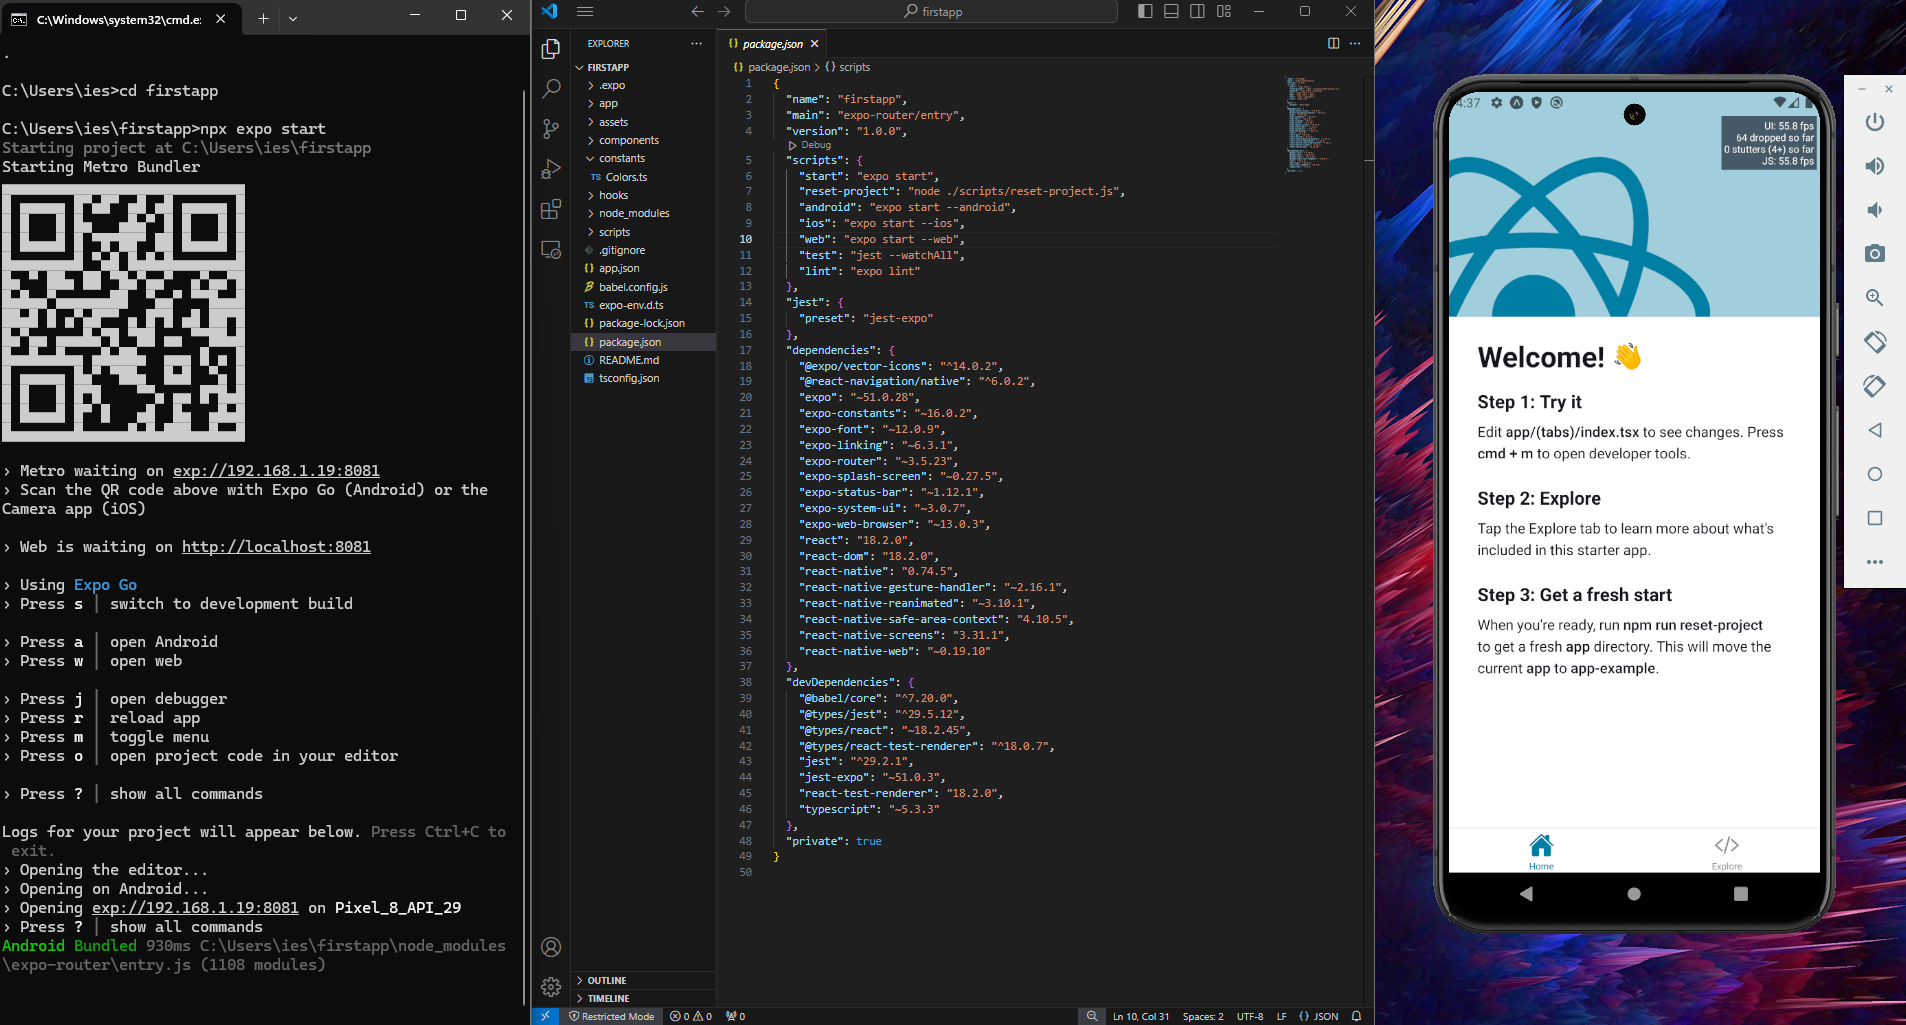
\includegraphics[width=11cm]{Inicio.png}
	\end{frame}
	\subsection{1.2. Dependencies al Package.json}
	\subsubsection{1.2.1. Package.json}
	\begin{frame}
		\centering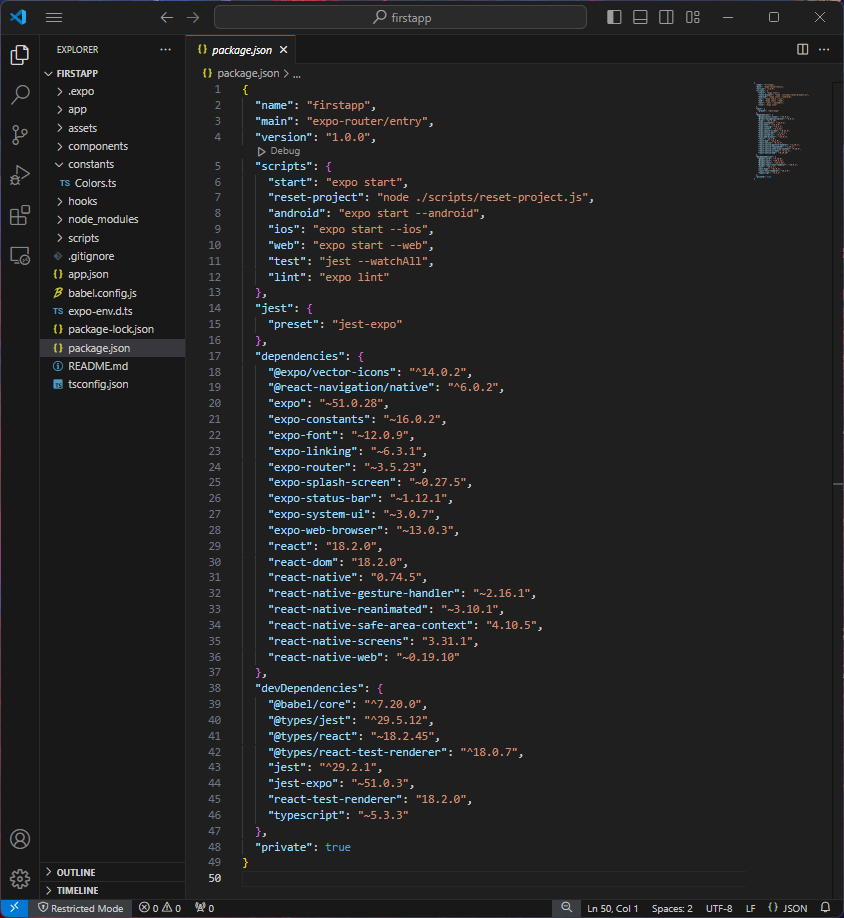
\includegraphics[height=8cm]{ProjectDefault01.png}
	\end{frame}
	\subsection{1.3. TabLayout, Index i Explore}
	\subsubsection{1.3.1. TabLayout}
	\begin{frame}
		\centering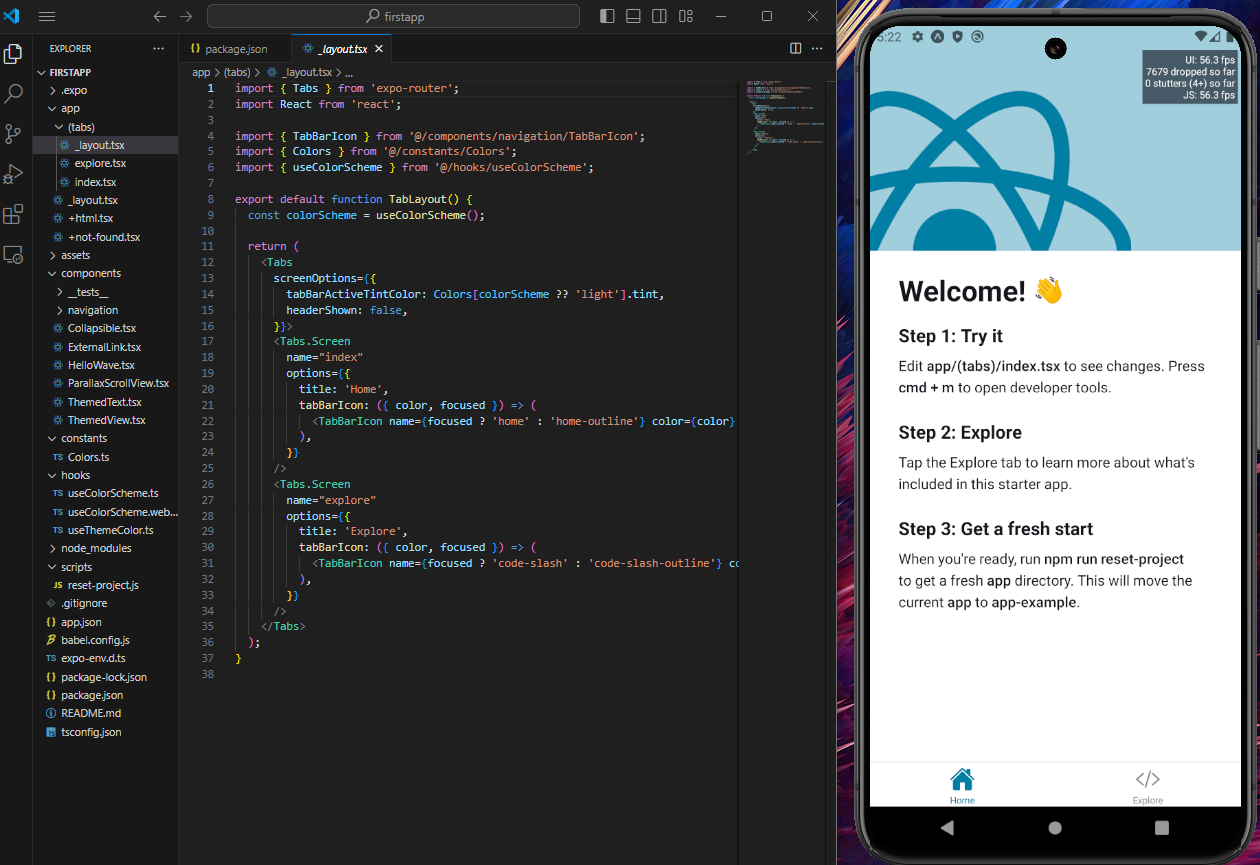
\includegraphics[width=10cm]{ProjectDefault02.png}
	\end{frame}
	\subsubsection{1.3.2. Index}
	\begin{frame}
		\centering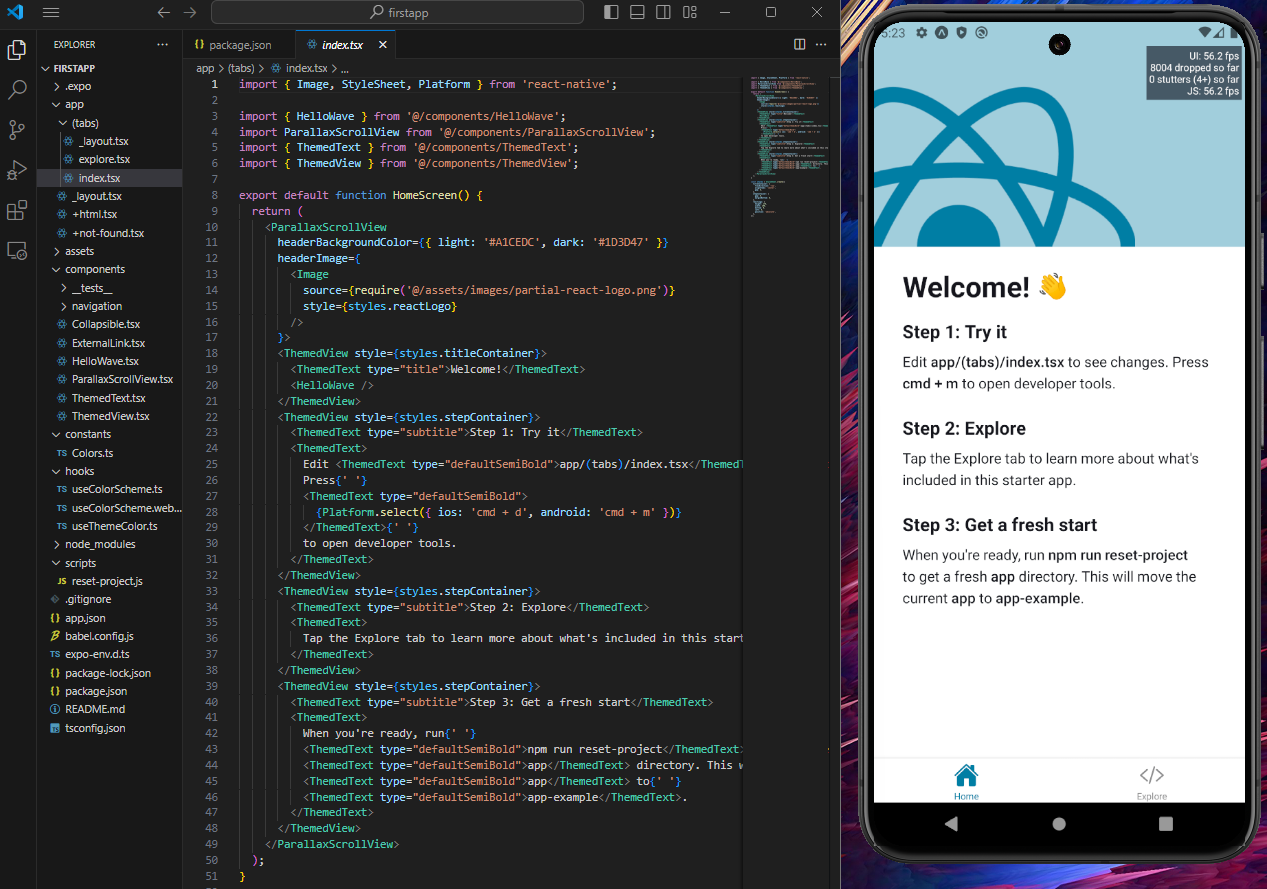
\includegraphics[width=10cm]{ProjectDefault03.png}
	\end{frame}
	\subsubsection{1.3.3. Explore}
	\begin{frame}
		\centering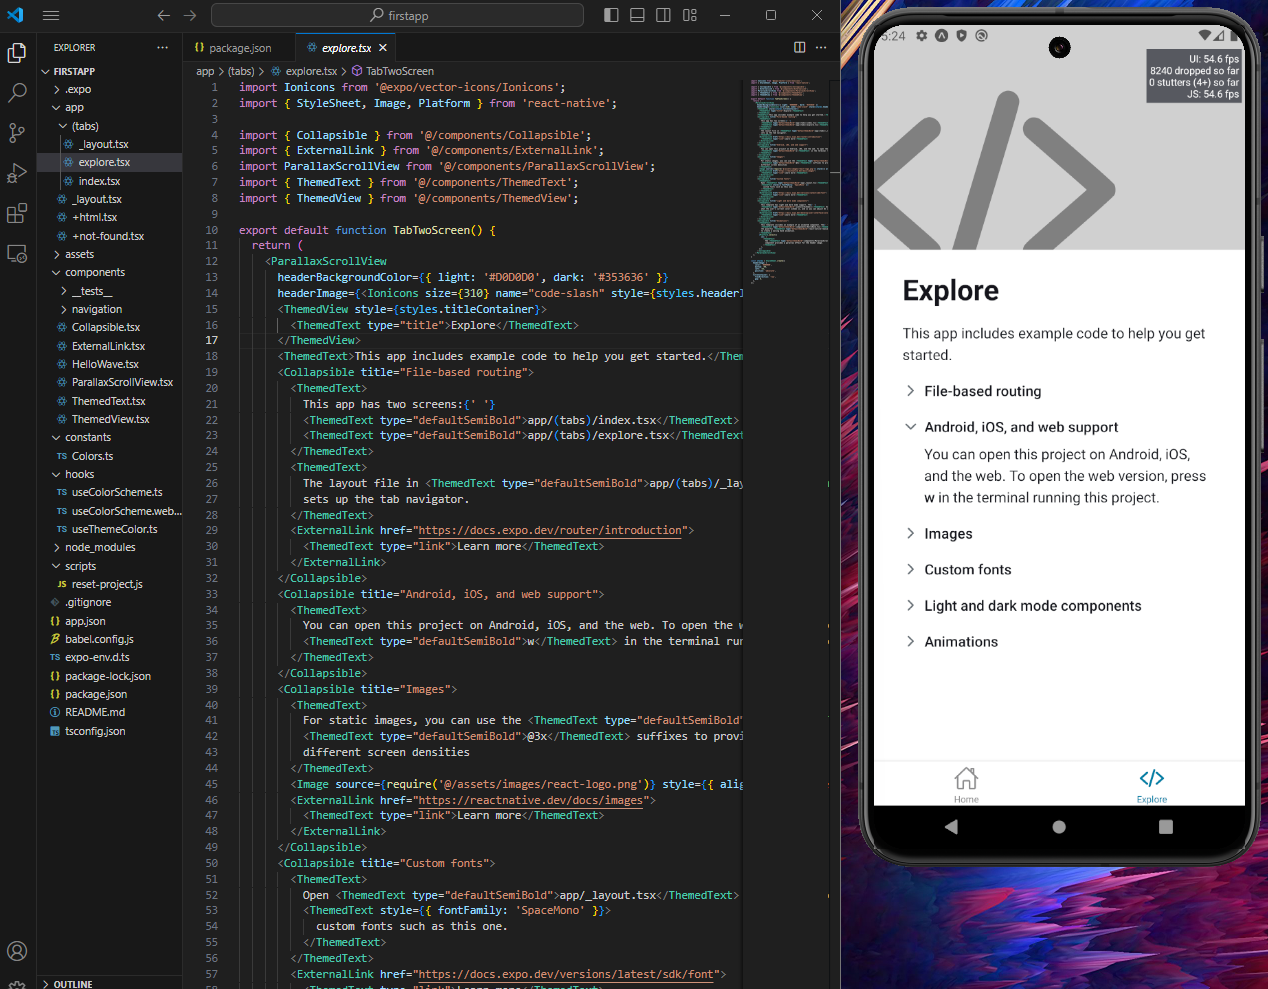
\includegraphics[width=10cm]{ProjectDefault04.png}
	\end{frame}
	\subsection{1.4. Constants com Recursos Fixos}
	\subsubsection{1.3.3. Constants}
	\begin{frame}
		\centering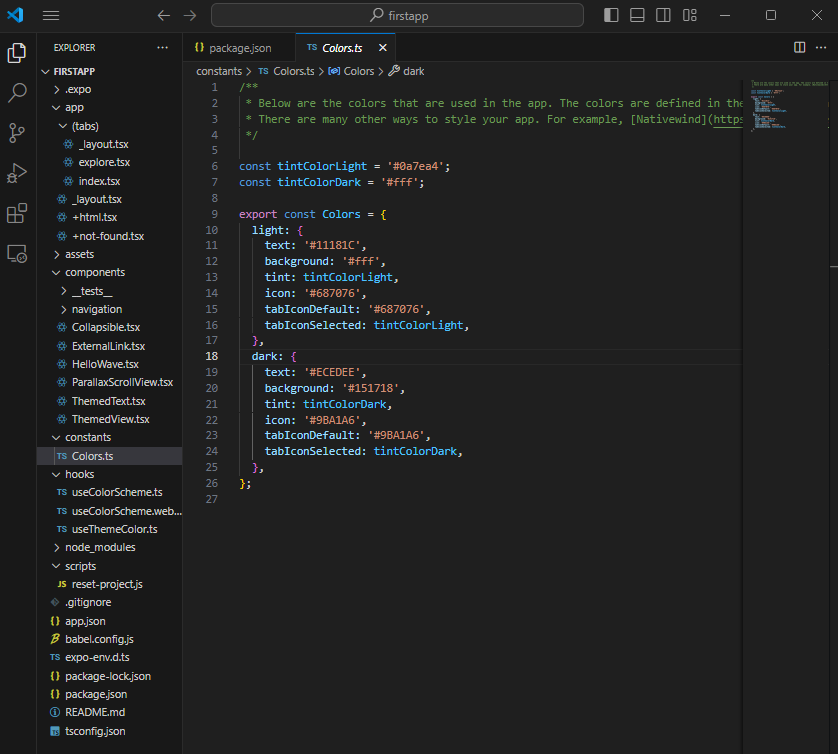
\includegraphics[width=7cm]{ProjectDefault05.png}
	\end{frame}
	\subsection{1.5. Components Utilitzats al Projecte}
	\subsubsection{1.5.1. Component HelloWave}
	\begin{frame}
		\centering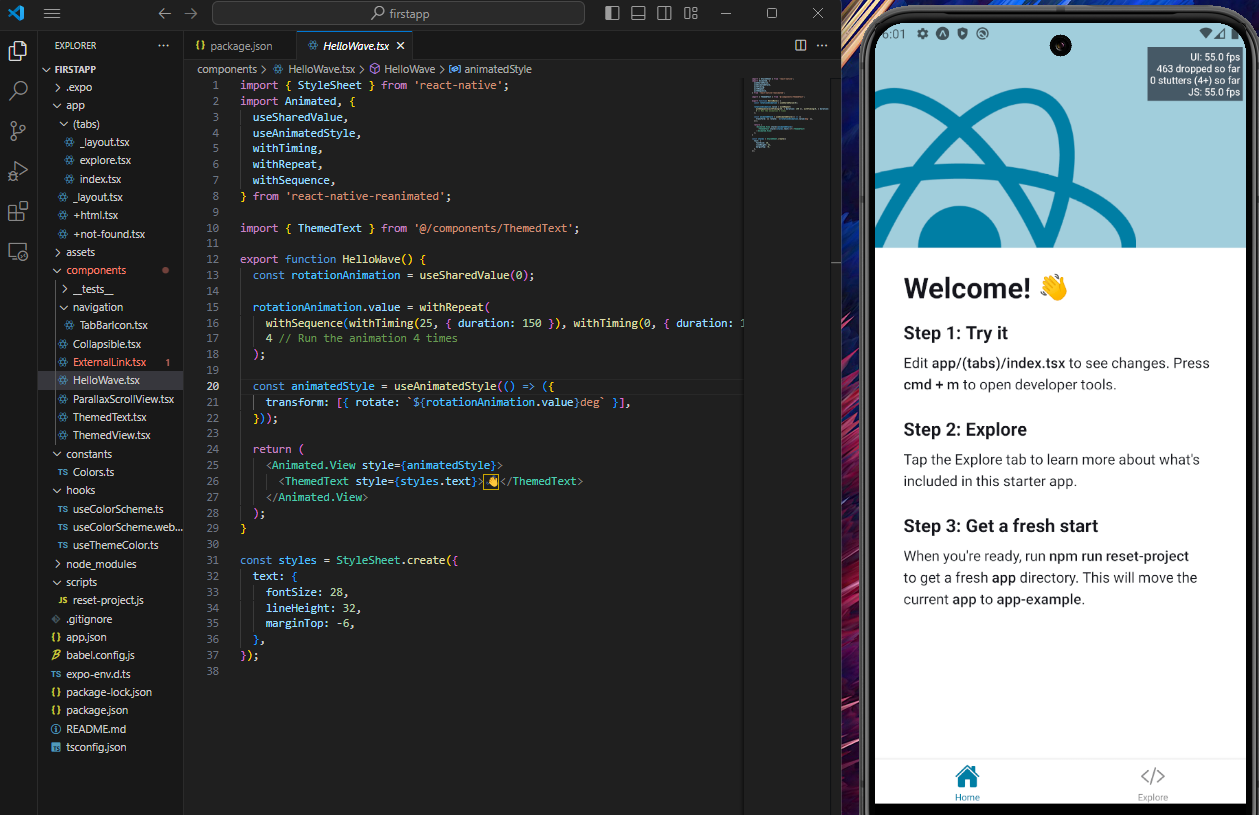
\includegraphics[width=10cm]{ProjectDefault06.png}
	\end{frame}
	\subsubsection{1.5.2. Component Collapsible}
	\begin{frame}
		\centering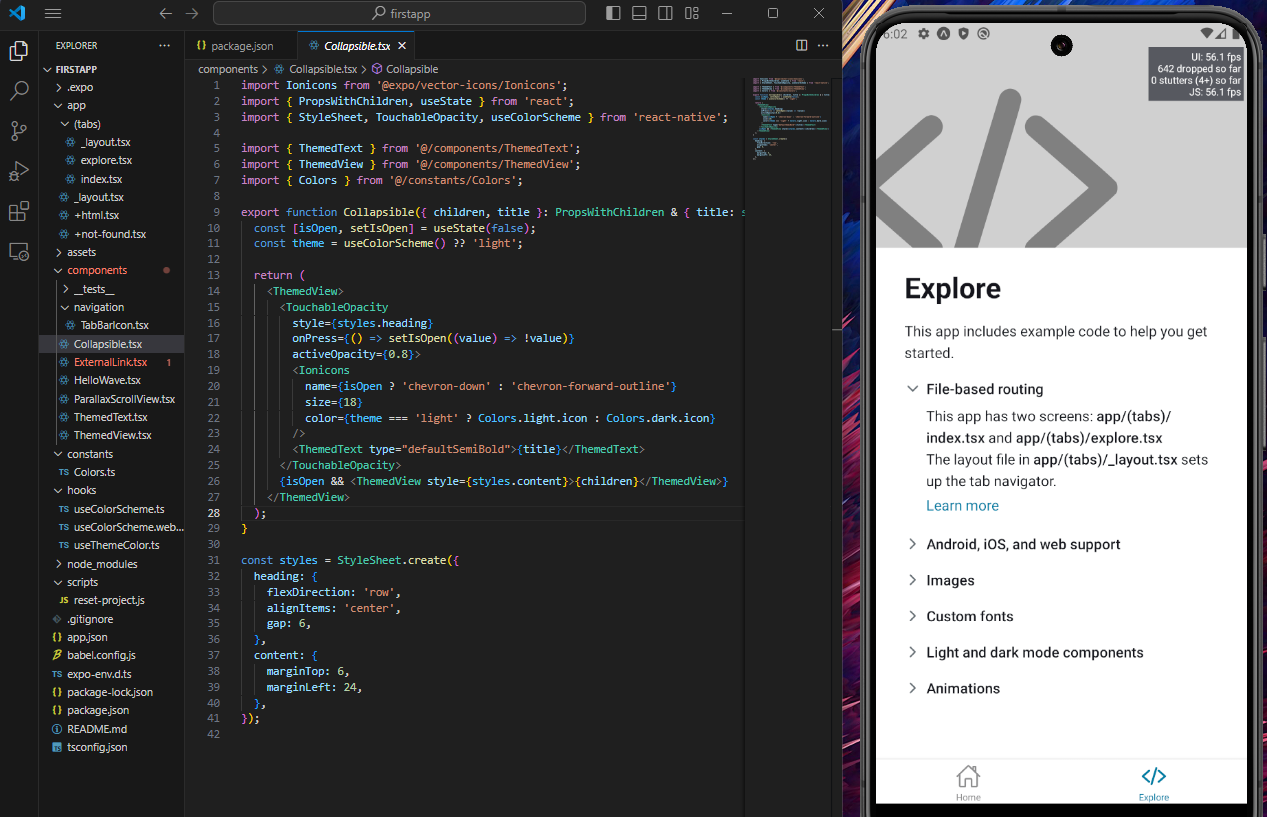
\includegraphics[width=10cm]{ProjectDefault07.png}
	\end{frame}
	\subsubsection{1.5.3. ComponentExternalLink}
	\begin{frame}
		\centering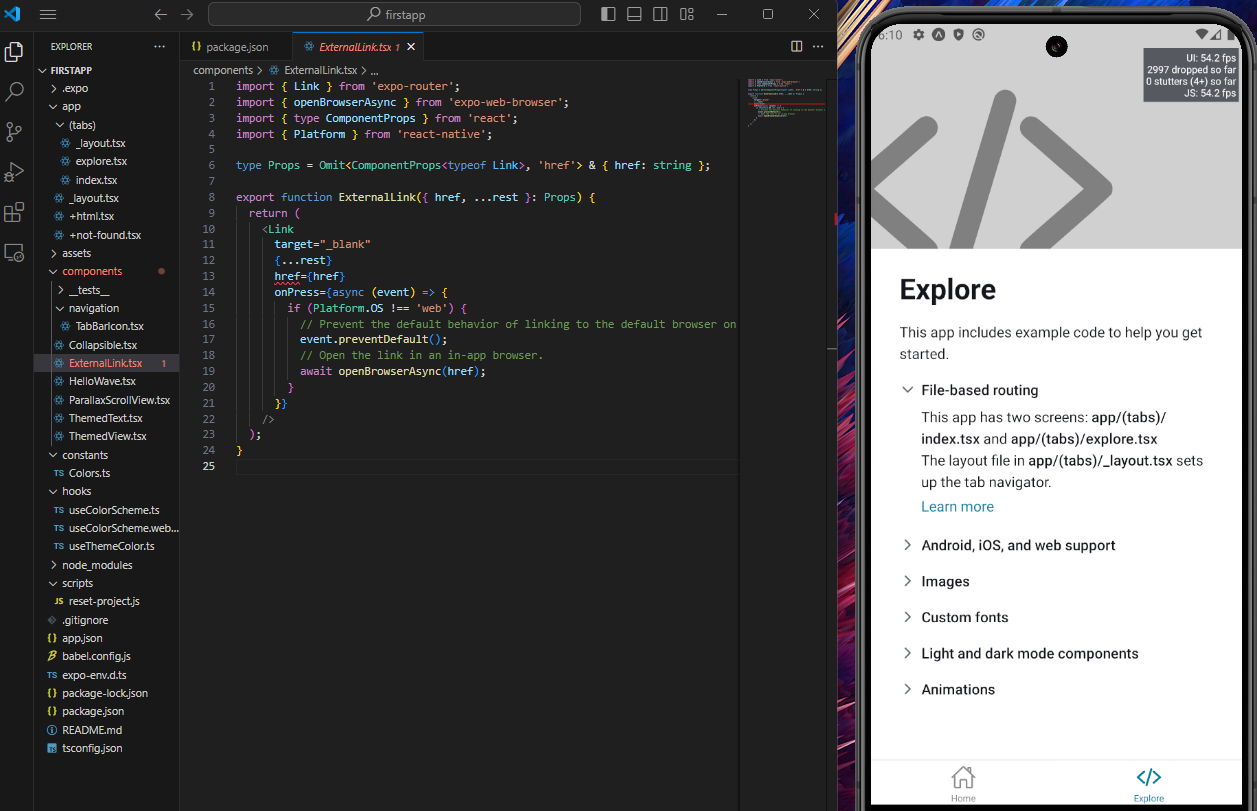
\includegraphics[width=10cm]{ProjectDefault09.png}
	\end{frame}
	\subsubsection{1.5.4. Component ThemedTest}
	\begin{frame}
		\centering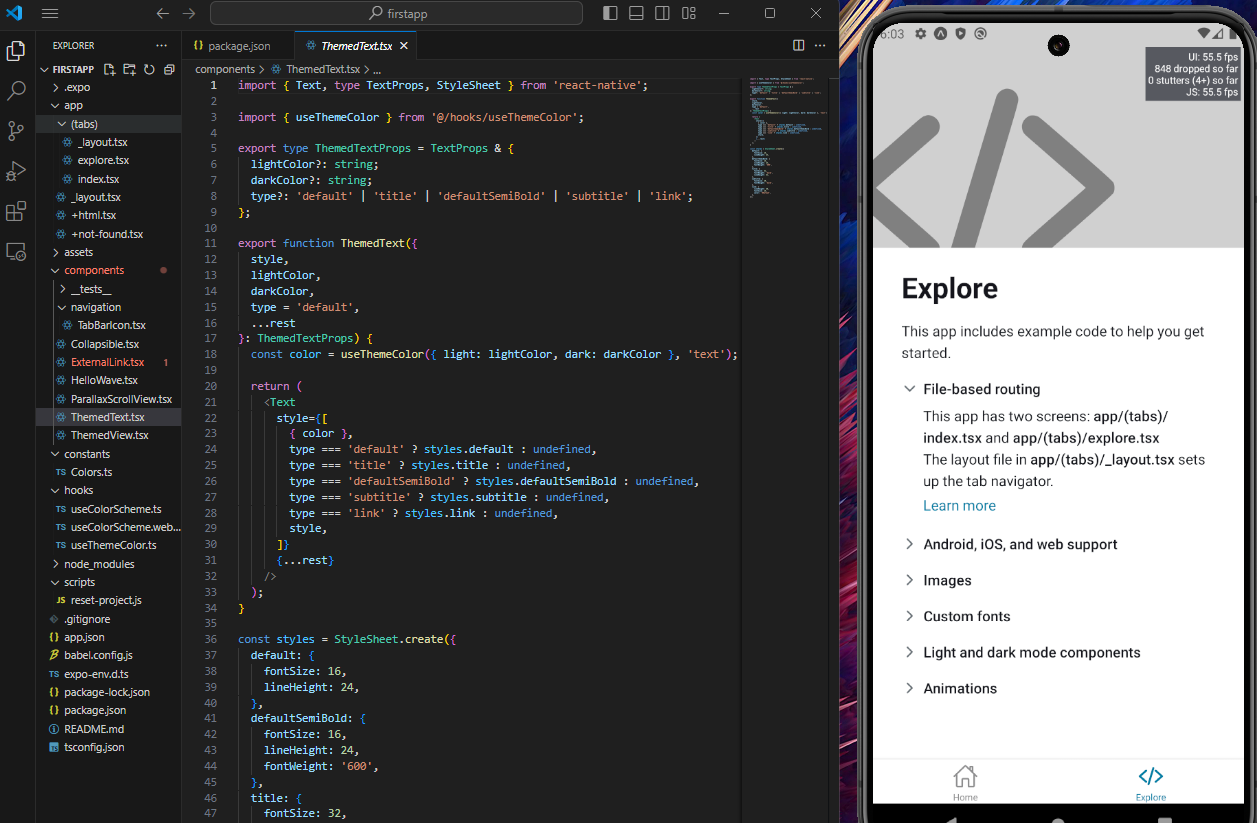
\includegraphics[width=10cm]{ProjectDefault08.png}
	\end{frame}
	\section{2. La Nostra Primera Aplicació React Native Bàsica}
	\subsection{2.0. Desenvolupament Online amb Snack Expo Dev}
	\subsubsection{2.0.1. Snack Expo Dev Project}
	\begin{frame}
		\centering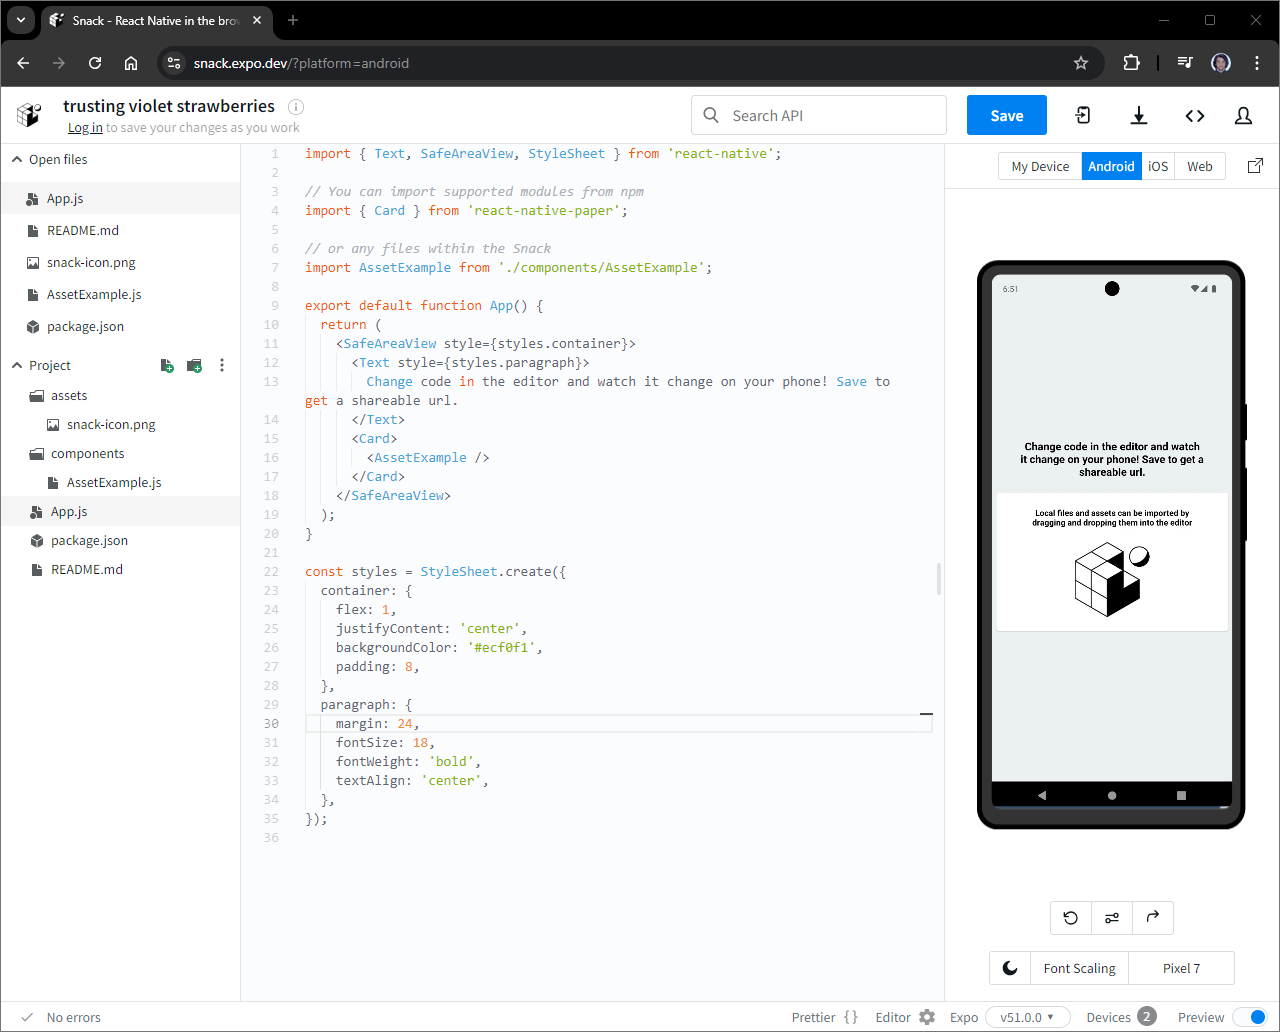
\includegraphics[width=10cm]{SnackExpoDev.png}
	\end{frame}
	\subsection{2.1. Iniciem un Projecte React Native en Blanc}
	\subsubsection{2.1.1. Comand per crear un Projecte React Native desde Zero}
	\begin{frame}
		\begin{block}{}
			Al iniciar els projectes podem escollir la plantilla inicial per l'aplicació que vulguem desenvolupar.
		\end{block}
		\centering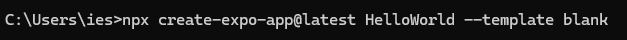
\includegraphics[width=10cm]{ProjectBlank01.png}\\
	\end{frame}
	\subsubsection{2.1.2. Altres posibles plantilles per React Native}
	\begin{frame}
		\begin{block}{Altres possibles plantiles per React Native}
			Los mas comunes son los siguientes:
			\begin{itemize}
				\item \texttt{tabs} Projecte amb navegació de React Navigation.
				\item \texttt{blank-typescript} Plantilla buida amb TypeScript.
				\item \texttt{tabs-typescript} Plantilla amb React Navigation i TypeScript. 
				\item \texttt{minimal} Menys dependencies que \texttt{blank}.
				\item \texttt{bare-minimum} Plantilla que et permet tenir accés directe a la configuració nativa per a Android i iOS (ideal per a integracions més personalitzades)
				\item Busqueu per les comunitats d'internet.
			\end{itemize}
		\end{block}
	\end{frame}
	\subsubsection{2.1.3. Plantilles Personalitzades desde GitHub}
	\begin{frame}
		\begin{block}{Plantilles Personalitzades desde GitHub}
			Expo té un enfocament minimalista, per això solen centrar-se en plantilles com blank, tabs i les variants amb TypeScript.
			\begin{center}
				
\includegraphics[width=10cm]{TemplatePersonalizadoGitHub.png}
			\end{center}		
			A més, és possible crear i utilitzar plantilles personalitzades allotjades a GitHub o repositoris locals. Per a això, pots especificar la URL del repositori de GitHub o altres en lloc de fer servir un nom predefinit als templates d'Expo.
		\end{block}
	\end{frame}
	\subsubsection{2.1.4. Iniciem el Projecte en Blanc i Veiem les Opcions}
	\begin{frame}
		\centering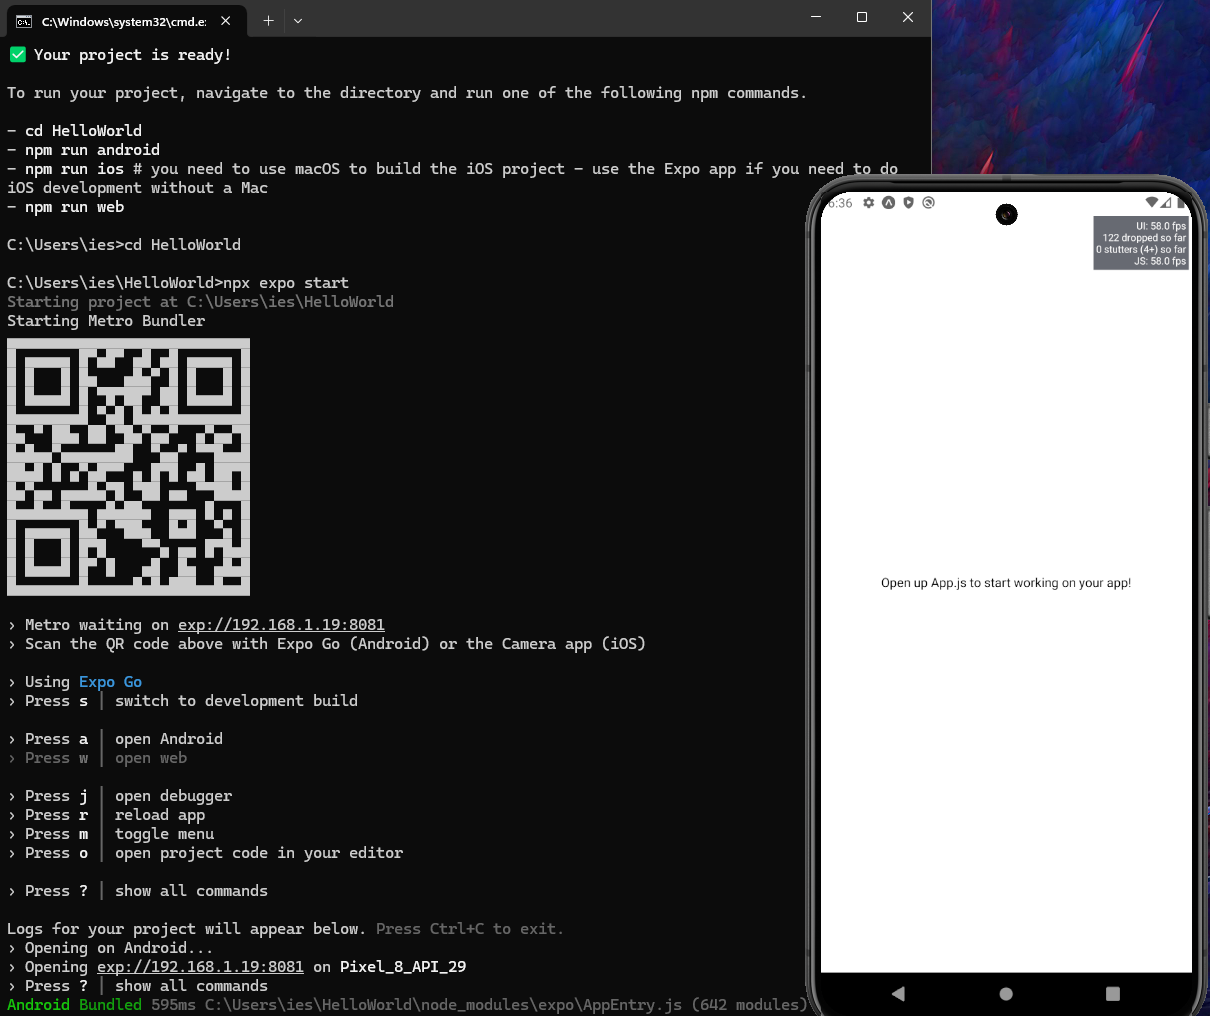
\includegraphics[width=9cm]{ProjectBlank02.png}\\
	\end{frame}
	\subsubsection{2.1.5. Projecte en blanc amb un Text dintre d'una View}
	\begin{frame}
		\centering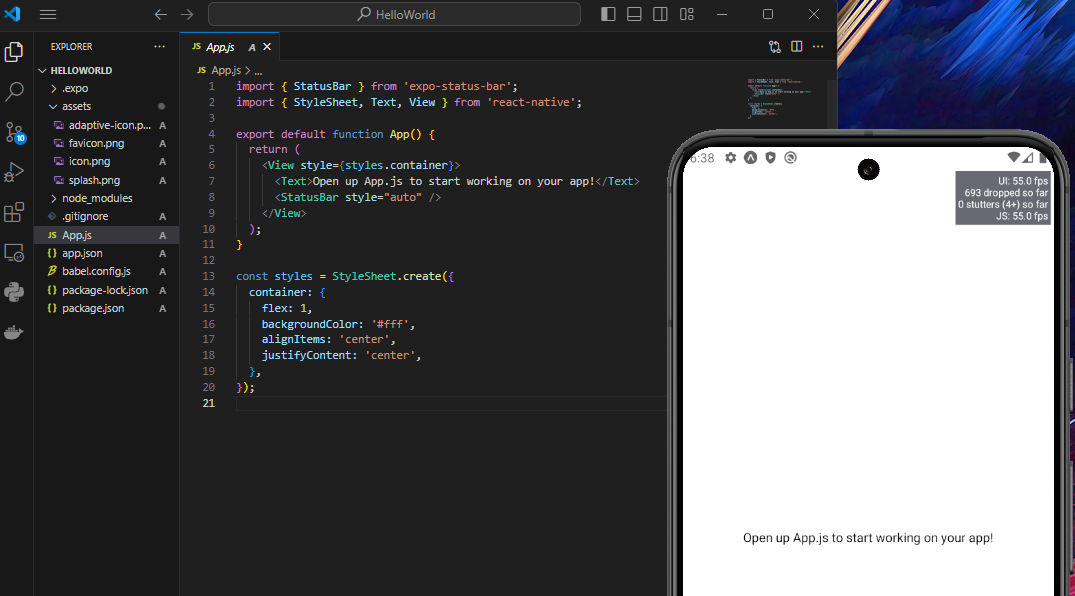
\includegraphics[width=11cm]{ProjectBlank03.png}\\
	\end{frame}
	\subsubsection{2.1.6. Dependencies del Projecte en blanc}
	\begin{frame}
		\centering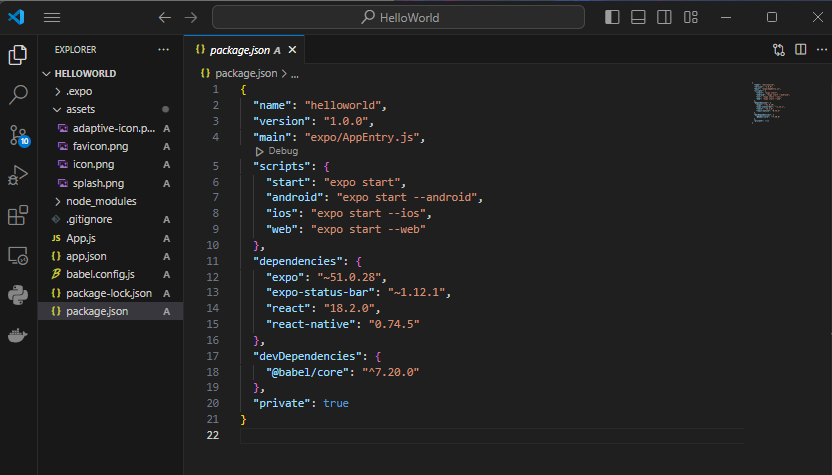
\includegraphics[width=11cm]{ProjectBlank05.png}\\
	\end{frame}
	\subsubsection{2.1.7. Afegim Dependencies Web al Projecte Blank}
	\begin{frame}
		\begin{block}{Afegim Dependencies Web al Projecte Blank}
			 Amb les següents comandes afegim les dependencies de \textbf{react-dom}, \textbf{react-native-web} i \textbf{@expo/metro-runtime}.
		\end{block}
		\centering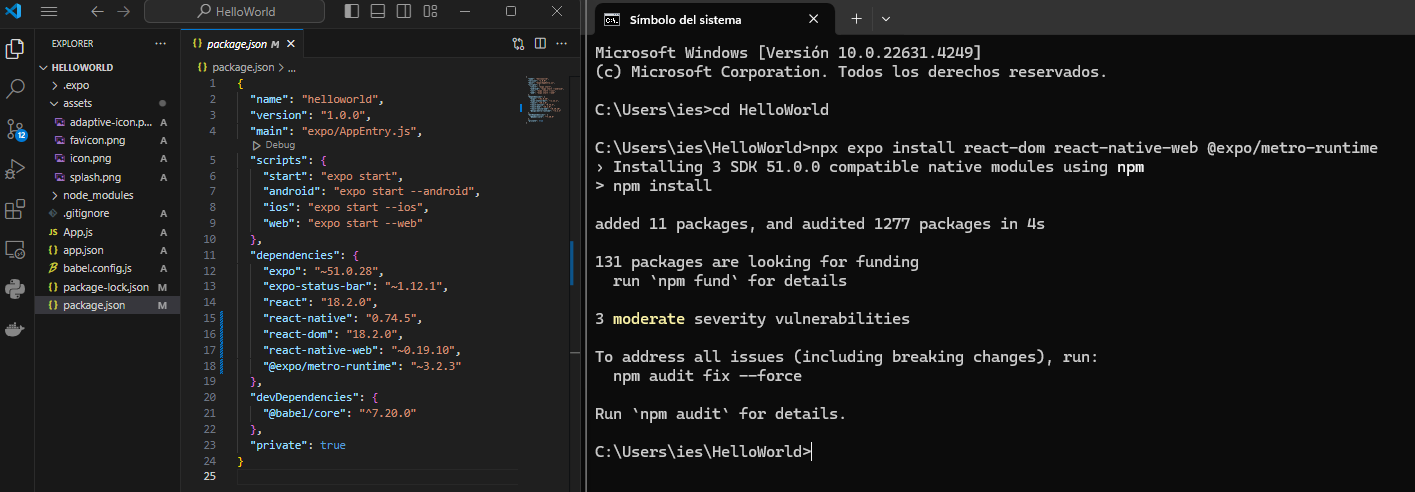
\includegraphics[width=11cm]{ProjectBlank06.png}\\
	\end{frame}
	\subsection{2.2. Components Bàsics}
	\subsubsection{2.2.0. Llista de Components Bàsics}
	\begin{frame}
		\begin{block}{Alguns componentes bàsics de React Native}
			\begin{table}[h!]
				\centering
				\begin{tabularx}{\textwidth}{|C{0.2\textwidth}|L{\dimexpr\textwidth-0.2\textwidth-2\tabcolsep-2\arrayrulewidth}}
					\hline
					Contenidors & 
					\textcolor{blue}{\texttt{View}} \ref{View}, 
					\textcolor{blue}{\texttt{SafeAreaView}} \ref{SafeAreaView}, 
					\textcolor{blue}{\texttt{Modal}} \ref{Modal},
					\textcolor{blue}{\texttt{KeyboardAvoidingView}} \ref{KeyboardAvoidingView} \\ \hline
					Text i dades & 
					\textcolor{blue}{\texttt{Text}} \ref{Text}, 
					\textcolor{blue}{\texttt{TextInput}} \ref{TextInput} \\ \hline
					Interaccions & 
					\textcolor{blue}{\texttt{Touchable}} \ref{Touchable},
					\textcolor{blue}{\texttt{Button}} \ref{Button},  
					\textcolor{blue}{\texttt{Pressable}} \ref{Pressable} \\ \hline
					Imatges & 
					\textcolor{blue}{\texttt{Image}} \ref{Image}, 
					\textcolor{blue}{\texttt{ImageBackground}} \ref{ImageBackground} \\ \hline
					Llistes & 
					\textcolor{blue}{\texttt{ScrollView}} \ref{ScrollView}, 
					\textcolor{blue}{\texttt{FlatList}} \ref{FlatList}, 
					\textcolor{blue}{\texttt{SectionList}} \ref{SectionList}, 
					\textcolor{blue}{\texttt{RefreshControl}} \ref{RefreshControl} \\ \hline
					Indicadors & 
					\textcolor{blue}{\texttt{ActivityIndicator}} \ref{ActivityIndicator} \\ \hline
					Altres visual & 
					\textcolor{blue}{\texttt{StatusBar}}\ref{StatusBar}, 
					\textcolor{blue}{\texttt{Picker}}\ref{Picker}, 
					\textcolor{blue}{\texttt{Slider}}\ref{Slider},
					\textcolor{blue}{\texttt{Switch}}\ref{Switch}\\ \hline
				\end{tabularx}
			\end{table}
		\end{block}
	\end{frame}
	\subsubsection{2.2.1. View y Text}
	\label{View}\label{Text}
	\begin{frame}
		\begin{block}{\texttt{View}}
			\begin{itemize}
				\item Contenidor bàsic per a elements de la interfície.
				\item Funciona com el \texttt{div} a HTML.
				\item Utilitzat per organitzar la disposició dels elements.
			\end{itemize}
		\end{block}
		\begin{block}{\texttt{Text}}
			\begin{itemize}
				\item Per mostrar text a la pantalla.
				\item Permet estilitzar fonts, mides, colors, etc.
			\end{itemize}
		\end{block}
	\end{frame}
	\begin{frame}
		\centering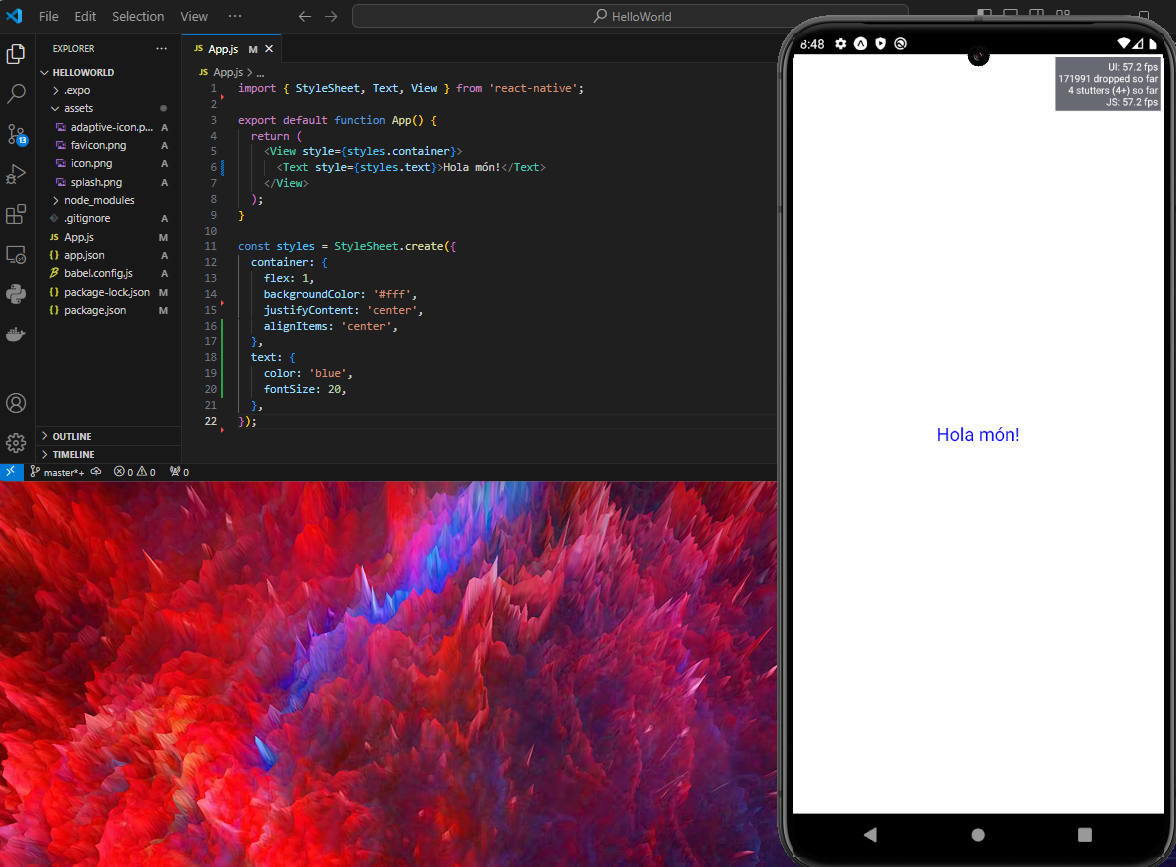
\includegraphics[width=11cm]{ProjectBlank07.png}
	\end{frame}
	\subsubsection{2.2.2. TextInput}
	\label{TextInput}
	\begin{frame}
		\begin{block}{\texttt{TextInput}}
			Per introduir dades des de l'usuari.
		\end{block}
		\centering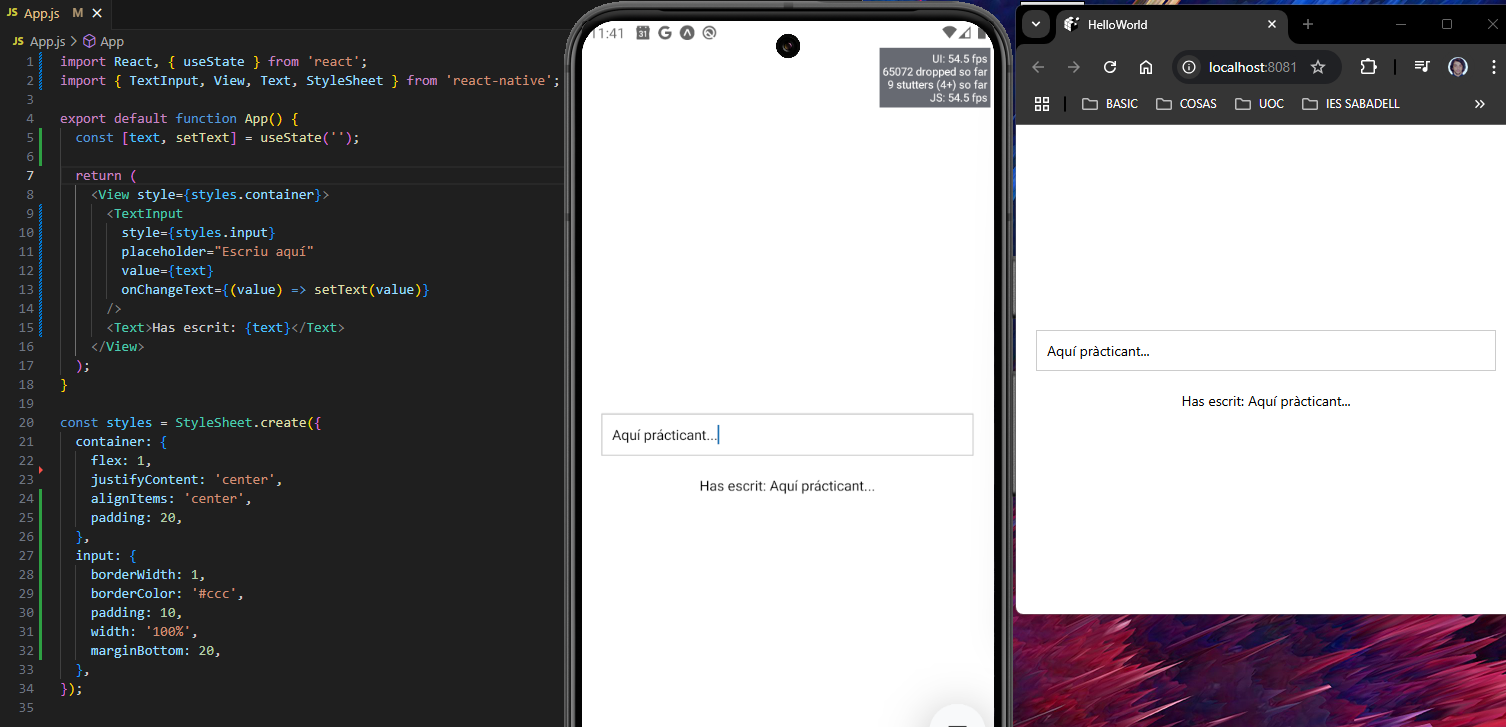
\includegraphics[width=11cm]{ProjectBlank31.png}
	\end{frame}
	\subsubsection{2.2.3. Touchable}
	\label{Touchable}
	\begin{frame}
		\begin{block}{\texttt{Touchable}}
			\begin{itemize}
				\item Per crear àrees interactives que responen a interaccions.
				\item Variants: \texttt{TouchableOpacity}, \texttt{TouchableHighlight}, \texttt{TouchableWithoutFeedback}.
			\end{itemize}
		\end{block}
		\centering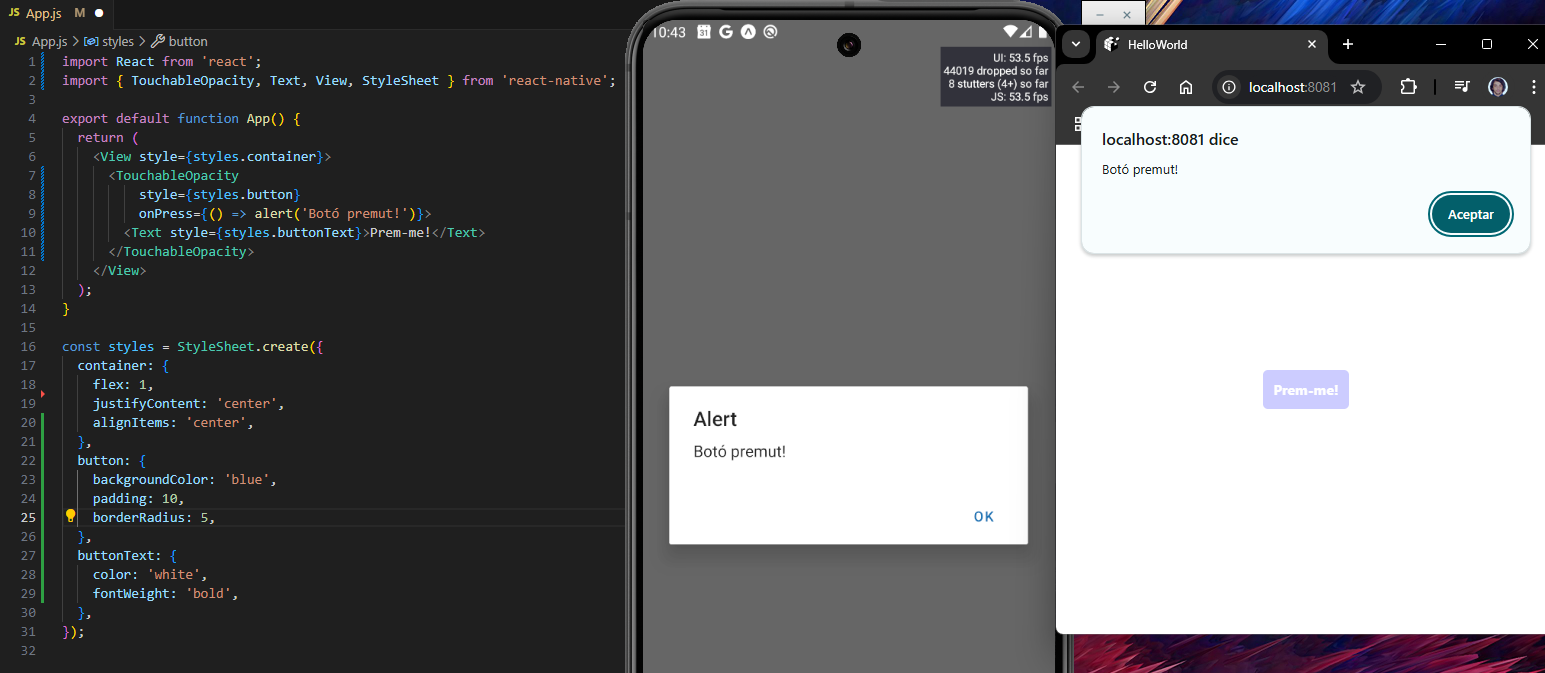
\includegraphics[width=11cm]{ProjectBlank30.png}
	\end{frame}
	\subsubsection{2.2.3. Button, Pressable}
	\label{Button}\label{Pressable}
	\begin{frame}
		\begin{block}{\texttt{Button}}
			\begin{itemize}
				\item Té estilització limitada (només el color de fons es pot personalitzar amb la propietat \texttt{color}).
				\item Utilitza \texttt{onPress} per gestionar l'acció en prémer el botó.
				\item És ideal per accions senzilles o quan no necessites personalització visual.
			\end{itemize}
		\end{block}
		\begin{block}{\texttt{Pressable}}
			\begin{itemize}
				\item Component més modern i flexible que permet personalitzar completament el botó.
				\item Accepta estats com pressed per canviar l'estil quan es pressiona.
				\item És ideal quan necessites un botó amb estil únic o complex.
			\end{itemize}
		\end{block}
	\end{frame}
	\begin{frame}
		\centering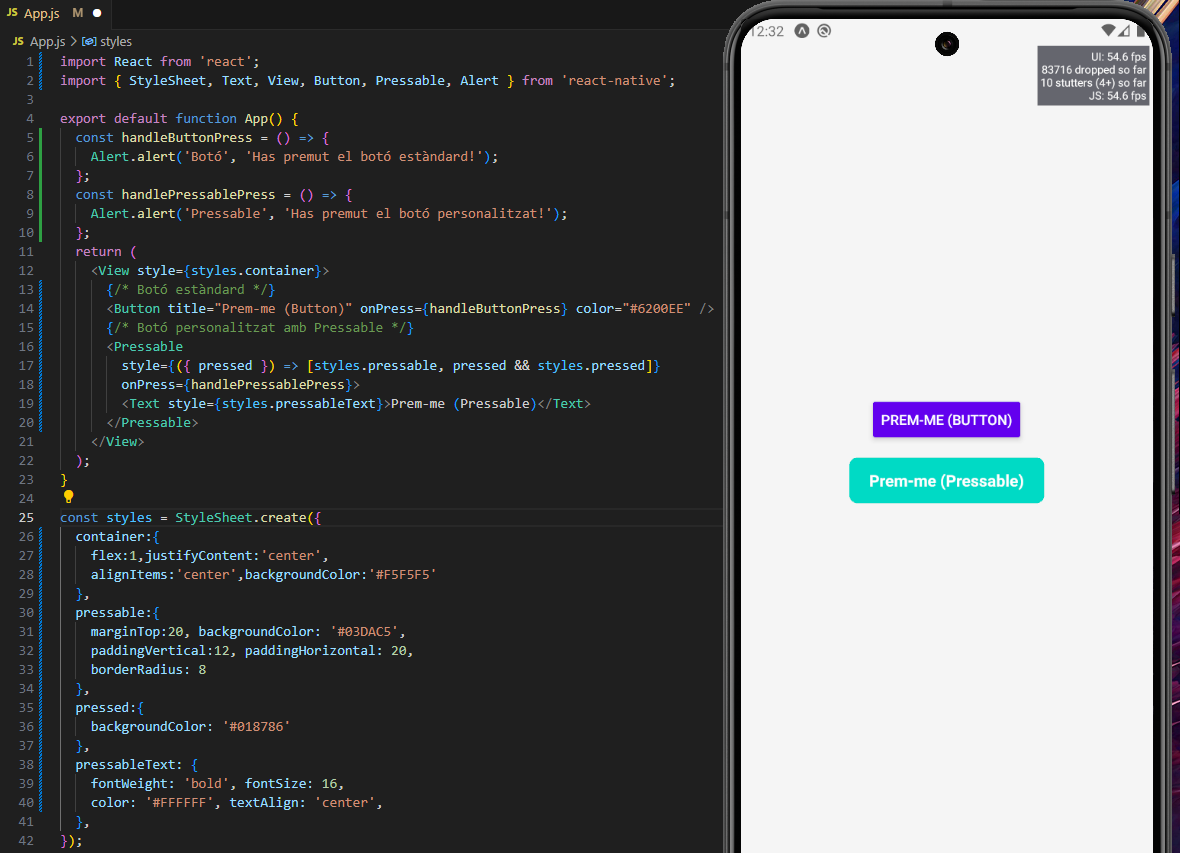
\includegraphics[width=11cm]{ProjectBlank33.png}
	\end{frame}
	\subsubsection{2.2.4. Image i ImageBackground}
	\label{Image}\label{ImageBackground}
	\begin{frame}
		\begin{block}{\texttt{Image} i \texttt{ImageBackground}}
			\texttt{Image} per mostrar imatges (localment o des d'URL).\\
			\texttt{ImageBackground} per establir una imatge com a fons.
		\end{block}
		\centering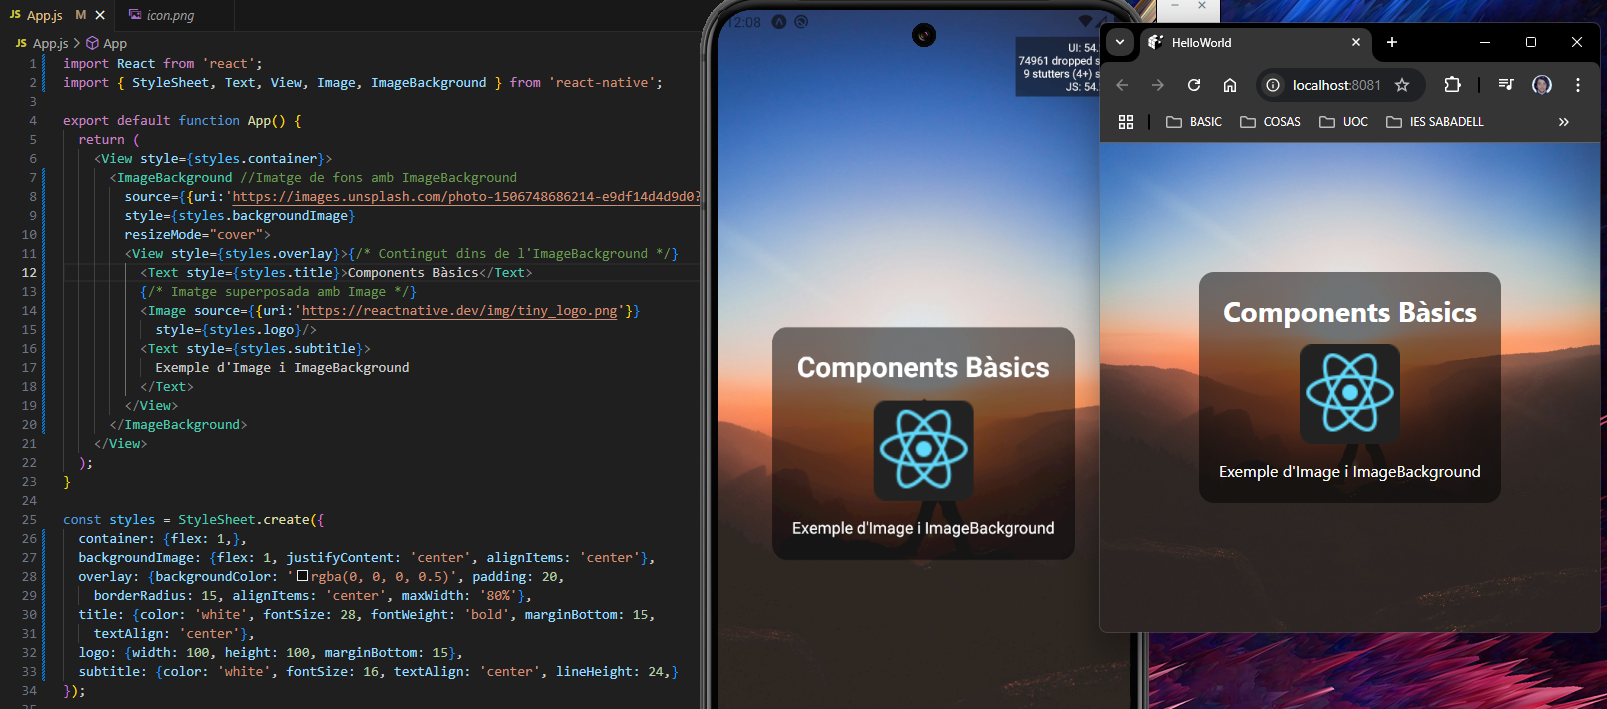
\includegraphics[width=11cm]{ProjectBlank32.png}
	\end{frame}
	\subsubsection{2.2.5. ScrollView}
	\label{ScrollView}
	\begin{frame}
	\begin{block}{\texttt{ScrollView}}
		\begin{itemize}
			\item Contenidor amb desplaçament vertical o horitzontal.
			\item Ideal per continguts variable que superen l'espai dispossat.
			\item Ofereix suport per gestos tàctils i funcionalitats com \texttt{pull-to-refresh}.
			\item Els items poden contenir \texttt{Text}, \texttt{Image} o \texttt{View}.
		\end{itemize}
	\end{block}
	\centering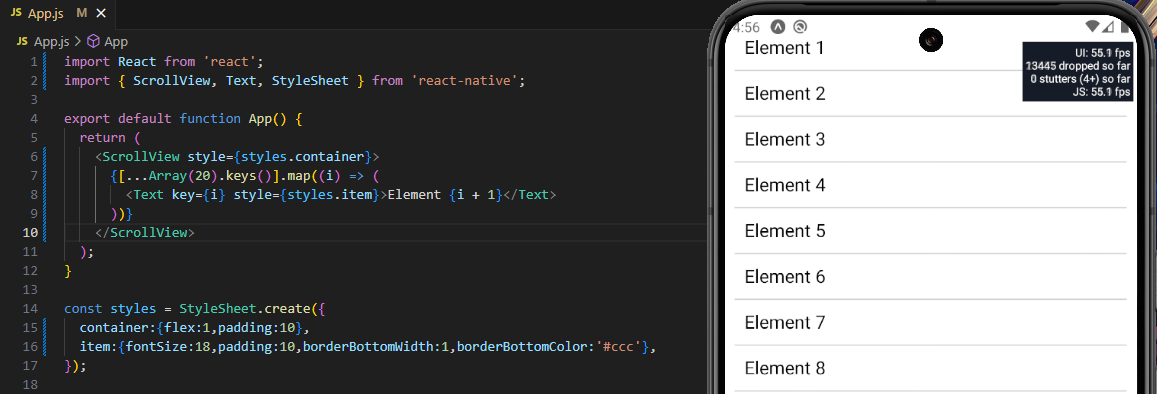
\includegraphics[width=11cm]{ProjectBlank37.png}
	\end{frame}
	
	\subsubsection{2.2.6. FlatList}
	\label{FlatList}
	\begin{frame}
		\begin{block}{\texttt{FlatList}}
			\begin{itemize}
				\item Per renderitzar grans llistes de forma optimitzada.
				\item Només renderitza els elements visibles.
			\end{itemize}
		\end{block}
		\centering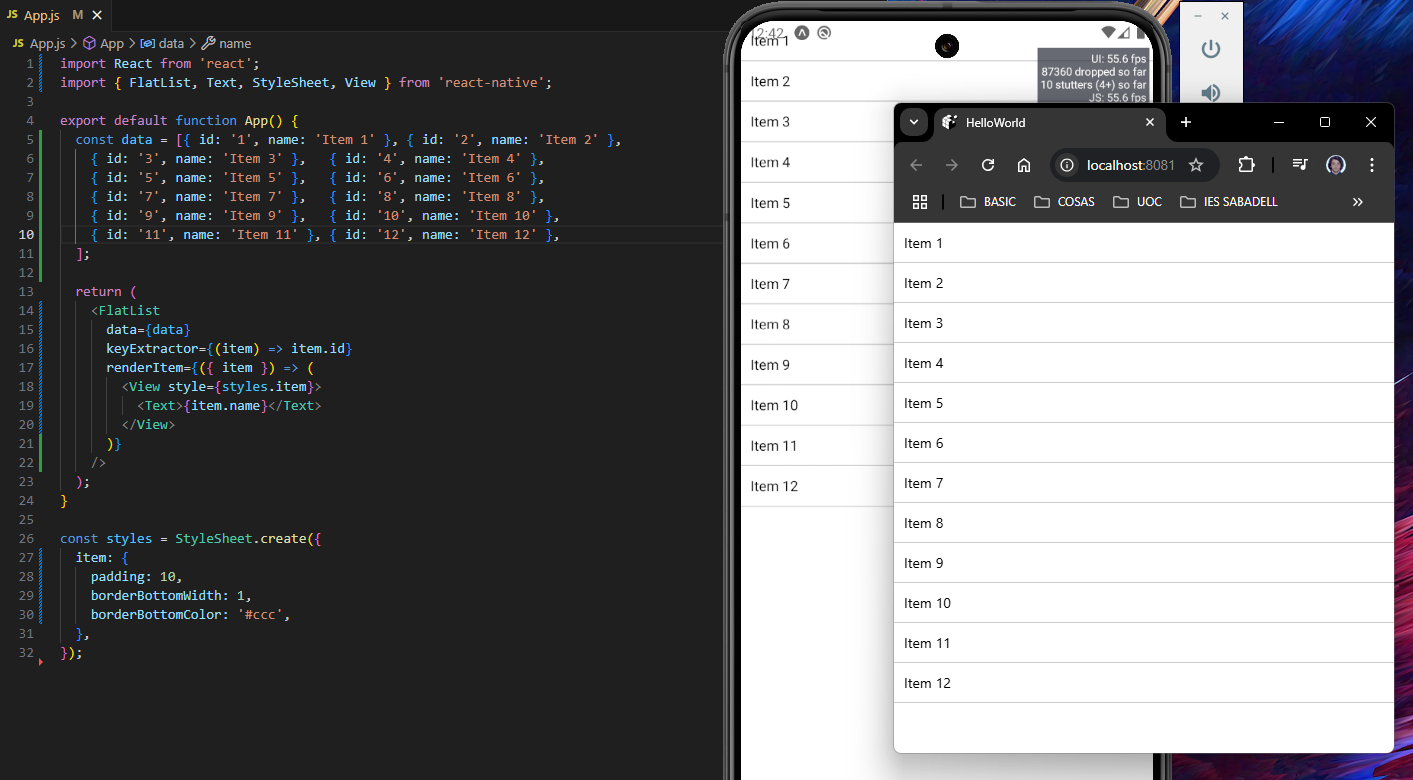
\includegraphics[width=11cm]{ProjectBlank34.png}
	\end{frame}
	\subsubsection{2.2.7. SectionList}
	\label{SectionList}
	\begin{frame}
		\begin{block}{\texttt{SectionList}}
			\begin{itemize}
				\item Similar a \texttt{FlatList}, però fent grups d'ítems (seccions).
				\item \texttt{sections} rep l'array d'objectes.
				\item Cada objecte té un (\texttt{title}) i un array (\texttt{data}).
				\item \texttt{keyExtractor}: Proporciona clau única per a cada ítem.
				\item \texttt{renderSectionHeader}: Renderitza els títols de secció.
				\item \texttt{renderItem}: Defineix com es mostrarà cada ítem. 
			\end{itemize}
		\end{block}
	\end{frame}
	\begin{frame}
		\centering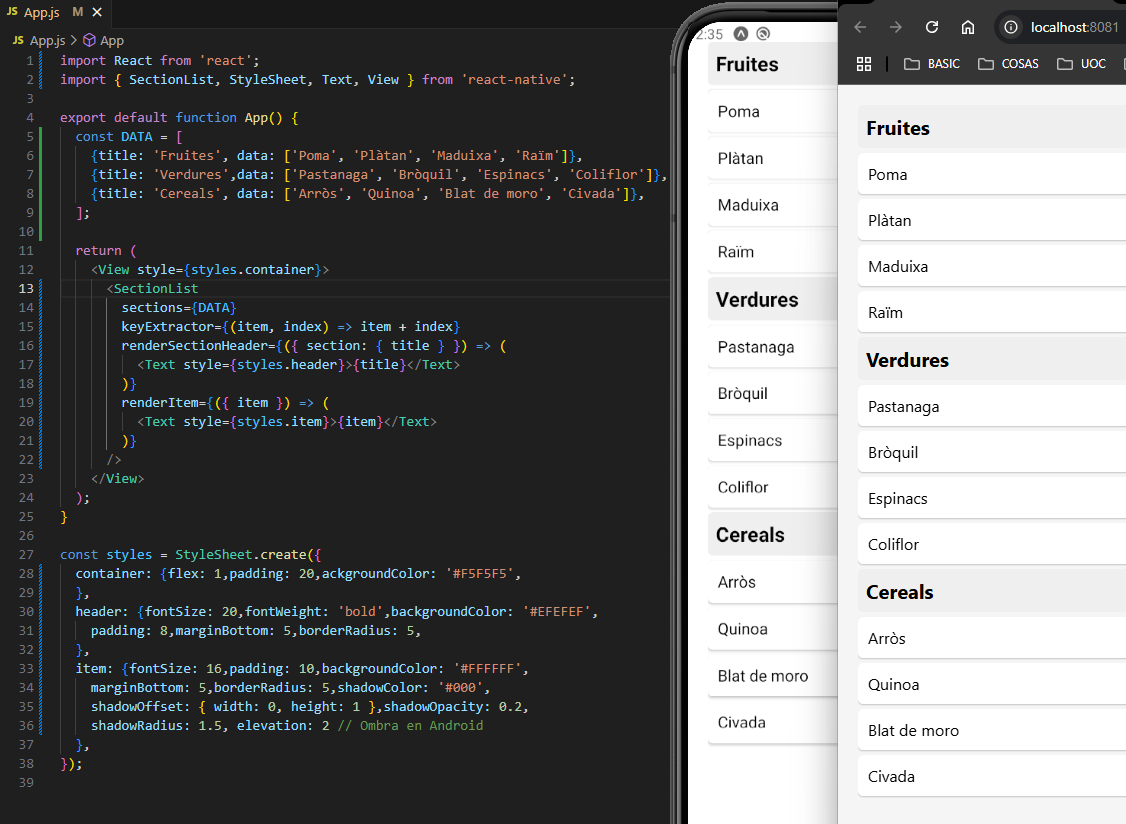
\includegraphics[width=11cm]{ProjectBlank35.png}
	\end{frame}
	\subsubsection{2.2.8. RefreshControl}
	\label{RefreshControl}
	\begin{frame}
		\begin{block}{\texttt{RefreshControl}}
			\begin{itemize}
				\item Afegeix la funcionalitat de "\textbf{pull-to-refresh}" a \texttt{ScrollView} o \texttt{FlatList}.
				\item Indica visualment que s'està recarregant contingut.
				\item Es pot personalitzar el color i l'animació del refresc.
			\end{itemize}
			Funcionament del següent exemple:
			\begin{enumerate}
				\item Es fa el gest de "pull-to-refresh" des de dalt del contingut.
				\item Es veu l'indicador de càrrega mentre el refresc està actiu.
				\item Després de 2 segons, es genera un nou element a la llista.
				\item L'indicador desapareix quan s'ha completat el refresc.
			\end{enumerate}
		\end{block}
	\end{frame}
	\begin{frame}
		\centering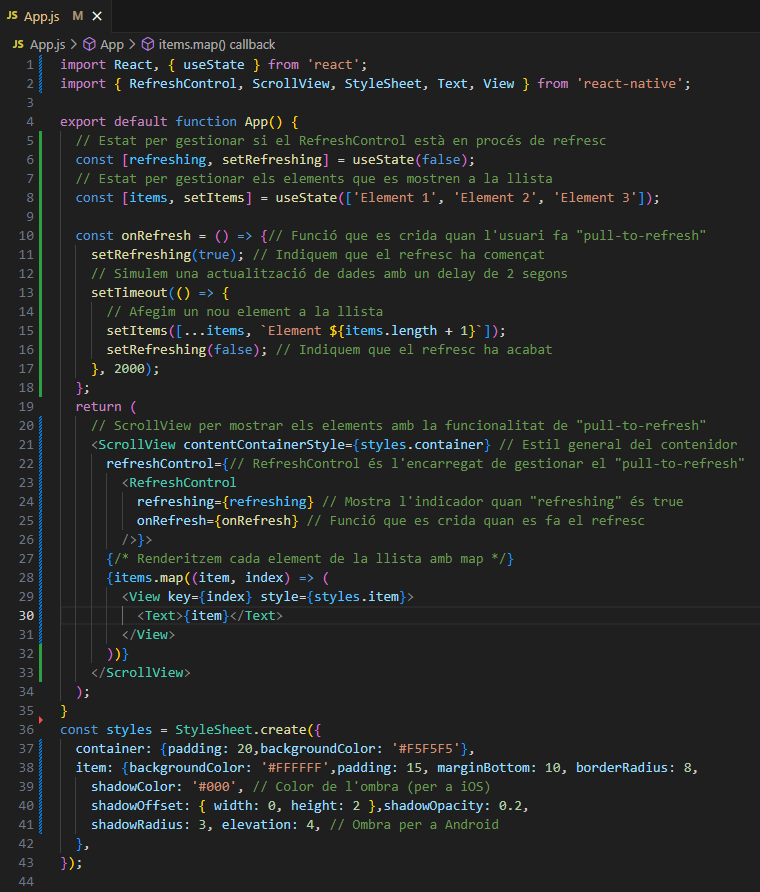
\includegraphics[width=7cm]{ProjectBlank36.png}
	\end{frame}
	\begin{frame}
		\centering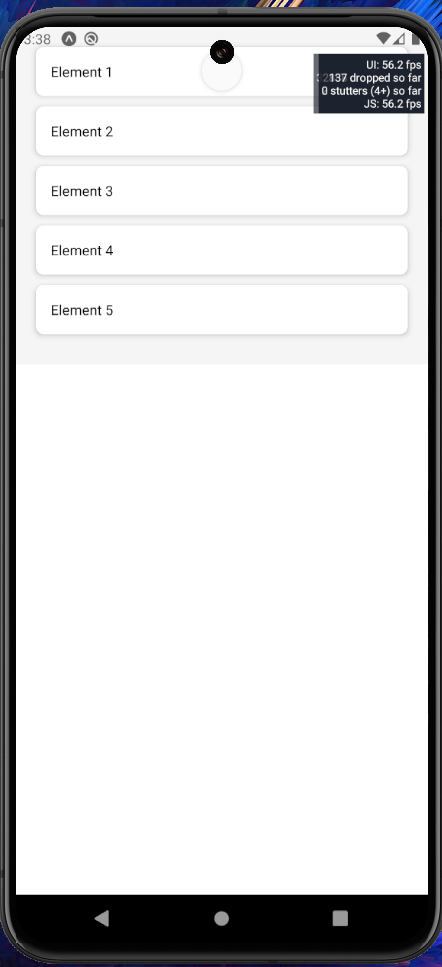
\includegraphics[height=11cm]{ProjectBlank38.png}
		\centering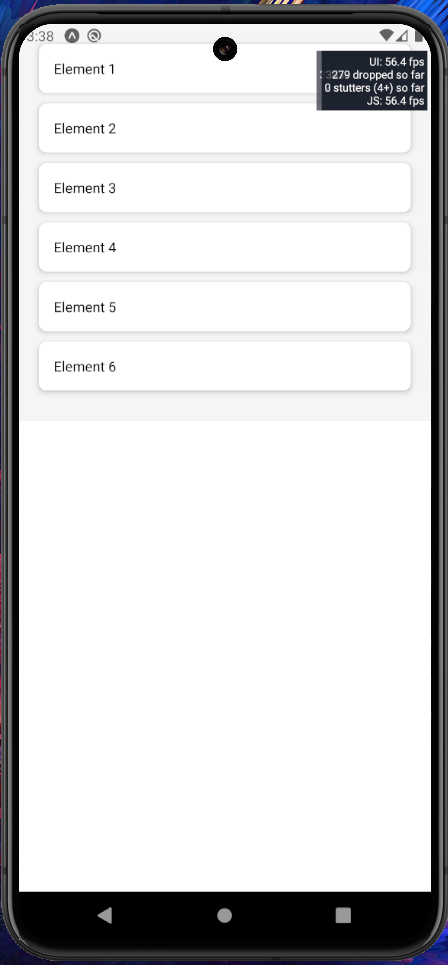
\includegraphics[height=11cm]{ProjectBlank39.png}
	\end{frame}
	\subsubsection{2.2.9. Modal}
	\label{Modal}
	\begin{frame}
		\begin{block}{\texttt{Modal}}
			\begin{itemize}
				\item Mostra una finestra emergent a sobre de la interfície.
				\item Ideal per a diàlegs, alertes o confirmacions.
				\item Inclou suport per animacions com \texttt{slide}, \texttt{fade} o \texttt{none}.
			\end{itemize}
			Funcionament del següent exemple:
			\begin{itemize}
				\item \texttt{useState}: Gestiona si el \texttt{Modal} és visible (\texttt{visible}).
				\item Propietats principals:
				\begin{itemize}
					\item \texttt{animationType}: Defineix l'animació del modal.
					\item \texttt{transparent}: Permet mostrar el fons semitransparent.
					\item \texttt{onRequestClose}: Gestió del tancament a Android.
				\end{itemize}
				\item Dos botons gestionen l'obertura i el tancament del \texttt{Modal}.
				\item El contenidor del modal (\texttt{modalView}) està estilitzat amb cantonades arrodonides i ombres.
			\end{itemize}
		\end{block}
	\end{frame}
	\begin{frame}
		\centering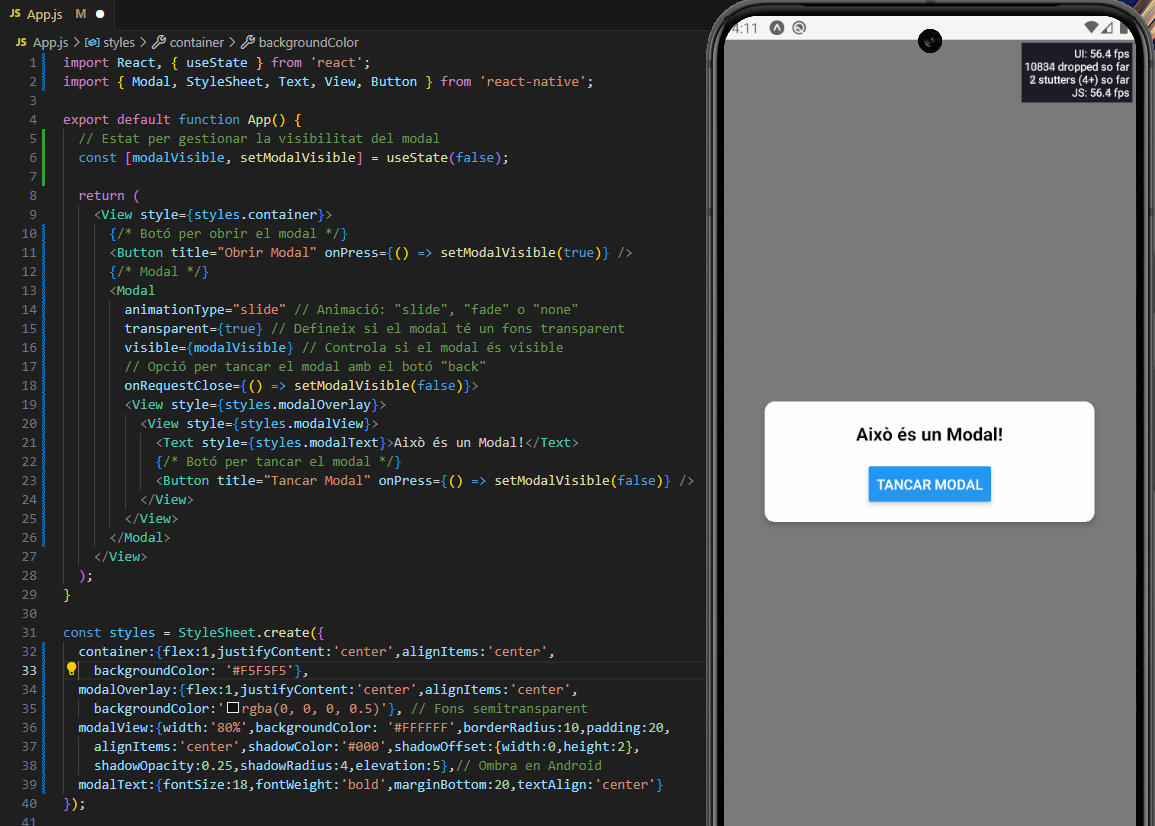
\includegraphics[width=11cm]{ProjectBlank40.png}
	\end{frame}
	\subsubsection{2.2.13. KeyboardAvoidingView}
	\label{KeyboardAvoidingView}
	\begin{frame}
		\begin{block}{\texttt{KeyboardAvoidingView}}
			\begin{itemize}
				\item Contenidor que ajusta els elements de la interfície quan el teclat virtual està actiu.
				\item Evita que els camps d'entrada quedin amagats sota el teclat.
				\item Configurable segons la plataforma (\texttt{padding} a iOS i \texttt{height} a Android).
				\item \texttt{behavior}: Controla el moviment del contingut quan apareix el teclat.
			\end{itemize}
		\end{block}
	\end{frame}
	\begin{frame}
		\centering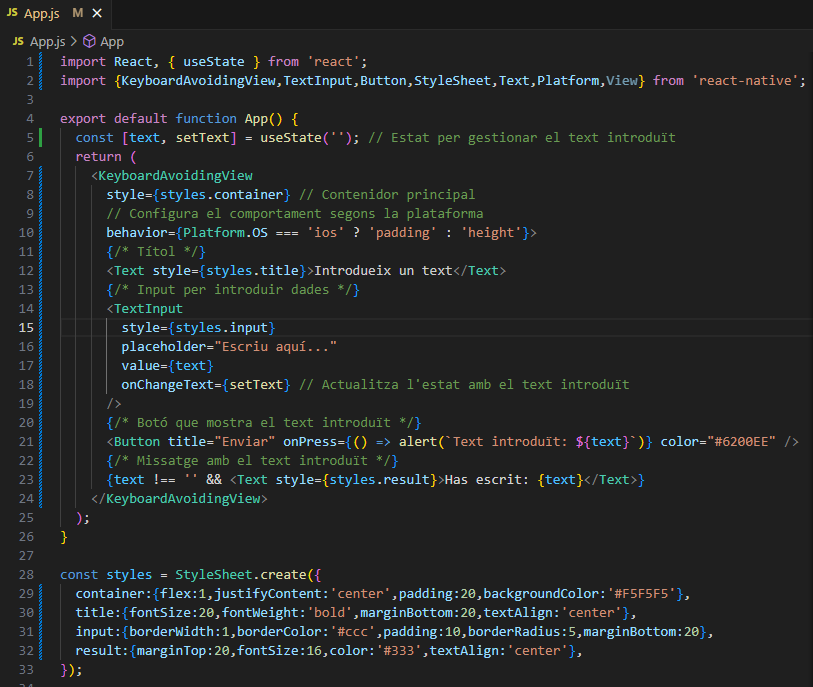
\includegraphics[width=9cm]{ProjectBlank42.png}
	\end{frame}
	\begin{frame}
		\centering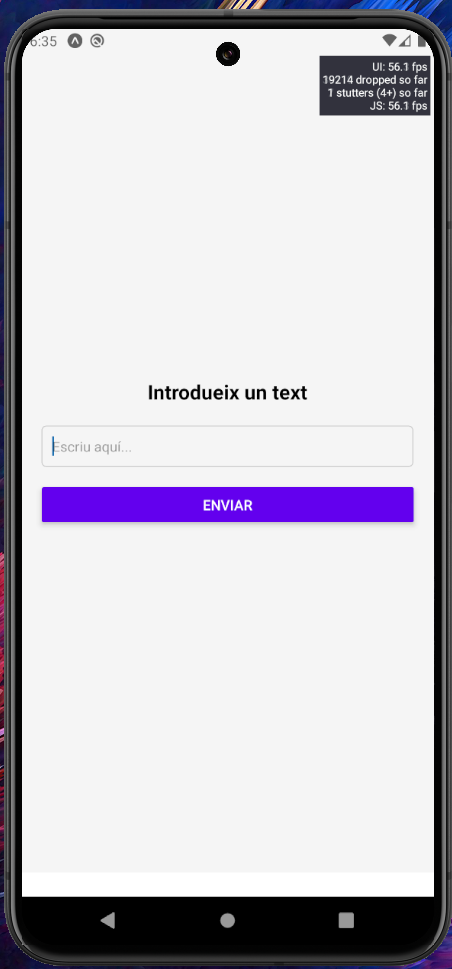
\includegraphics[height=8cm]{ProjectBlank44.png}
		\centering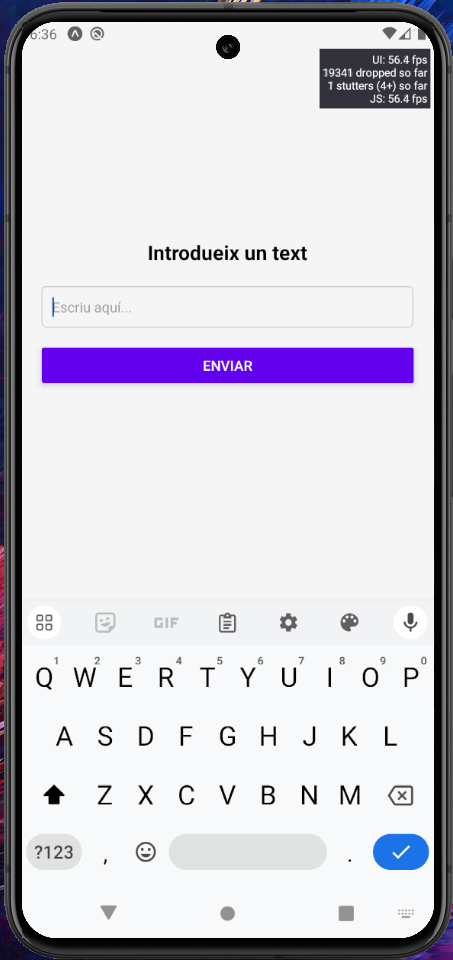
\includegraphics[height=8cm]{ProjectBlank45.png}
	\end{frame}
	\subsubsection{2.2.14. SafeAreaView}
	\label{SafeAreaView}
	\begin{frame}
		\begin{block}{\texttt{SafeAreaView}}
			\begin{itemize}
				\item Proporciona una àrea segura per mostrar contingut sense interferències del notch o la barra d'estat.
				\item Recomanat per a dispositius moderns amb dissenys sense marcs.
				\item Ajuda a garantir una millor experiència d'usuari.
			\end{itemize}
			A l'exemple el \texttt{SafeAreaView} conté el contingut dins de la zona protegida.
		\end{block}
	\end{frame}
	\begin{frame}
		\centering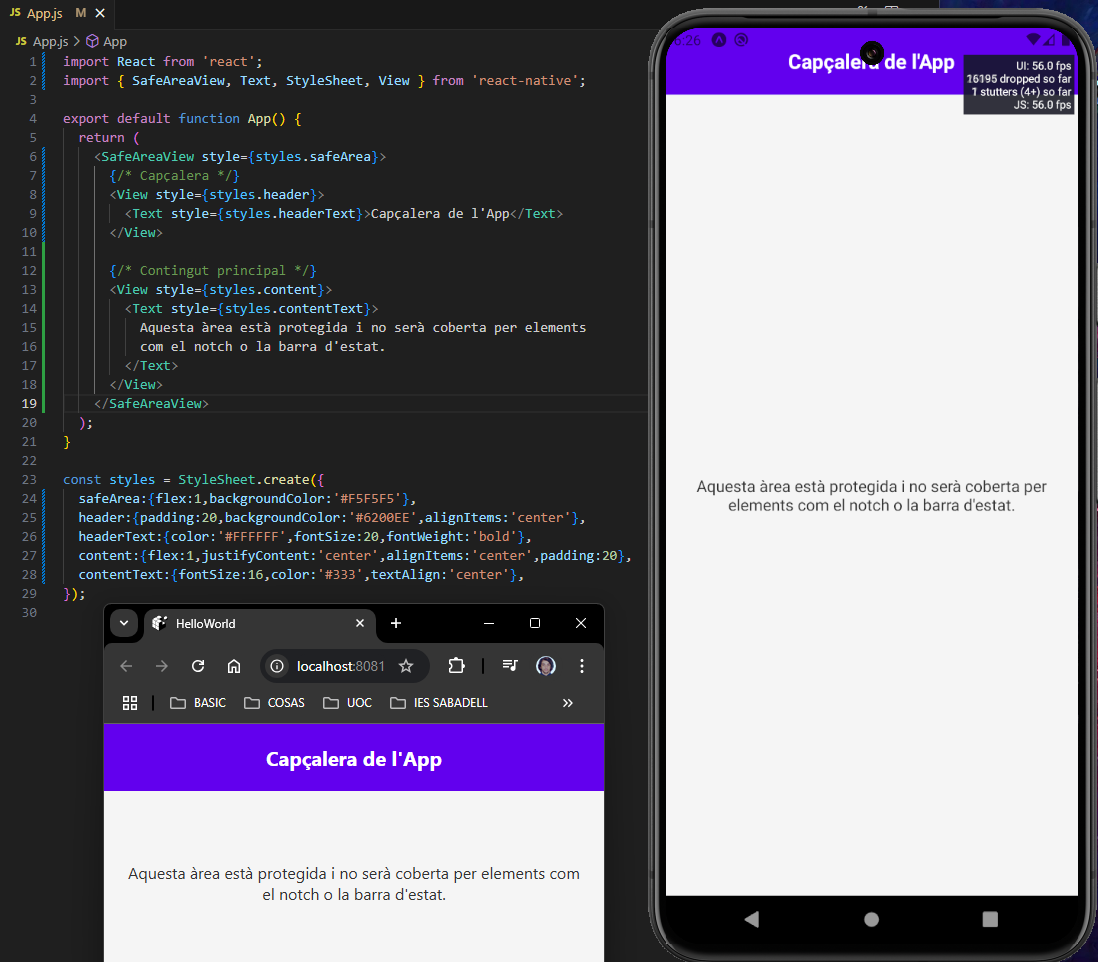
\includegraphics[width=9cm]{ProjectBlank43.png}
	\end{frame}
	\subsubsection{2.2.12. ActivityIndicator}
	\label{ActivityIndicator}
	\begin{frame}
		\begin{block}{\texttt{ActivityIndicator}}
			\begin{itemize}
				\item Mostra un indicador de càrrega (spinner).
				\item Es pot personalitzar amb mides i colors.
				\item Ideal per mostrar a l'usuari que hi ha una acció en curs.
			\end{itemize}
			Funcionament del següent exemple:
			\begin{itemize}
				\item \texttt{ActivityIndicator}: Mostra l'indicador segons \texttt{loading}
				\item Propietats personalitzables:
				\begin{itemize}
					\item \texttt{size}: Defineix la mida de l'indicador (\texttt{small} o \texttt{large}).
					\item \texttt{color}: Defineix el color de l'indicador.
				\end{itemize}
				\item Flux del codi:
				\begin{itemize}
					\item Amb el botó s'activa \texttt{startLoading}.
					\item \texttt{setTimeout} simula un procés de càrrega.
					\item Finalitzat el procés, \texttt{loading=false} i l'indicador bye.
				\end{itemize}
			\end{itemize}
		\end{block}
	\end{frame}
	\begin{frame}
		\centering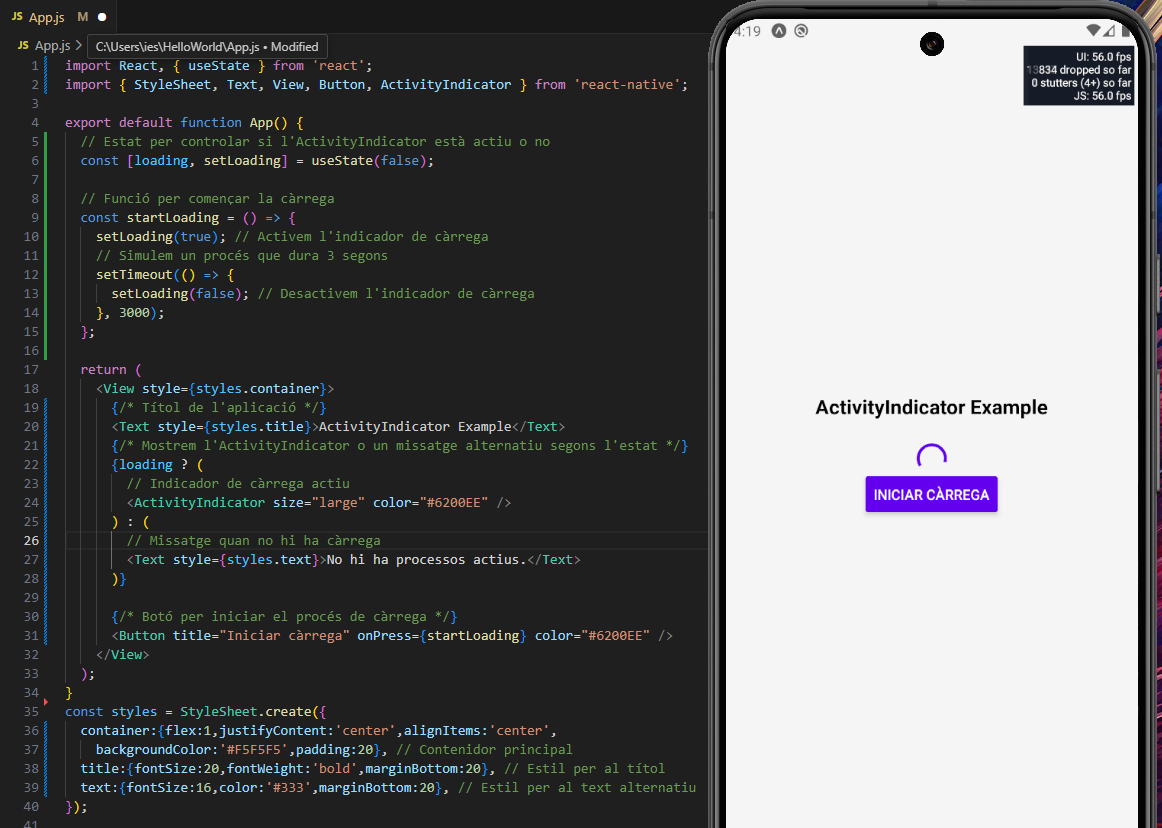
\includegraphics[width=11cm]{ProjectBlank41.png}
	\end{frame}
	\subsubsection{2.2.17. StatusBar}
	\label{StatusBar}
	\begin{frame}
		\begin{block}{\texttt{StatusBar}}
			\begin{itemize}
				\item Permet personalitzar la barra d'estat del dispositiu.
				\item Configurable amb estils com \texttt{light-content} o \texttt{dark-content}.
				\item Opció de mostrar o amagar la barra d'estat amb la propietat \texttt{hidden}.
			\end{itemize}
		\end{block}
	\end{frame}
	\begin{frame}
		\centering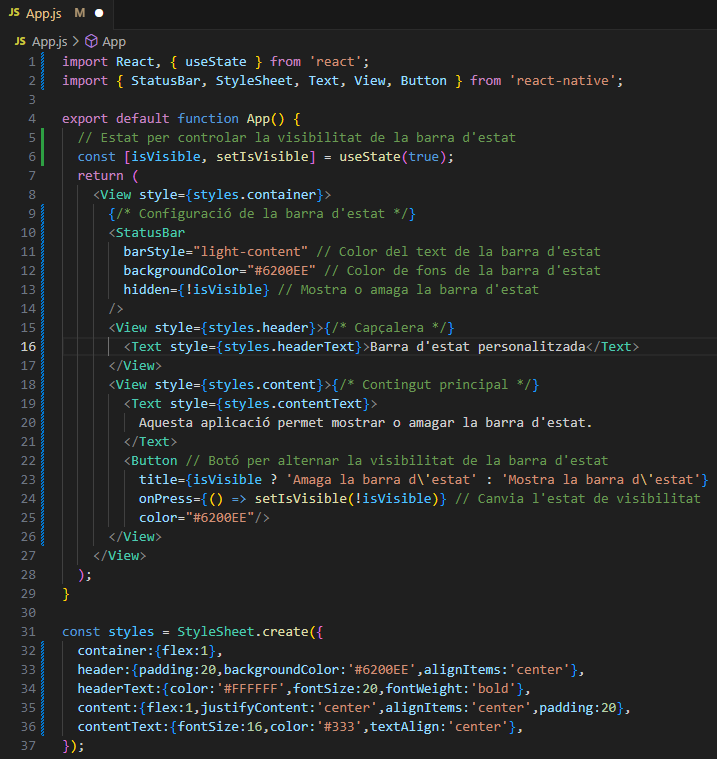
\includegraphics[width=9cm]{ProjectBlank46.png}
	\end{frame}
	\begin{frame}
		\centering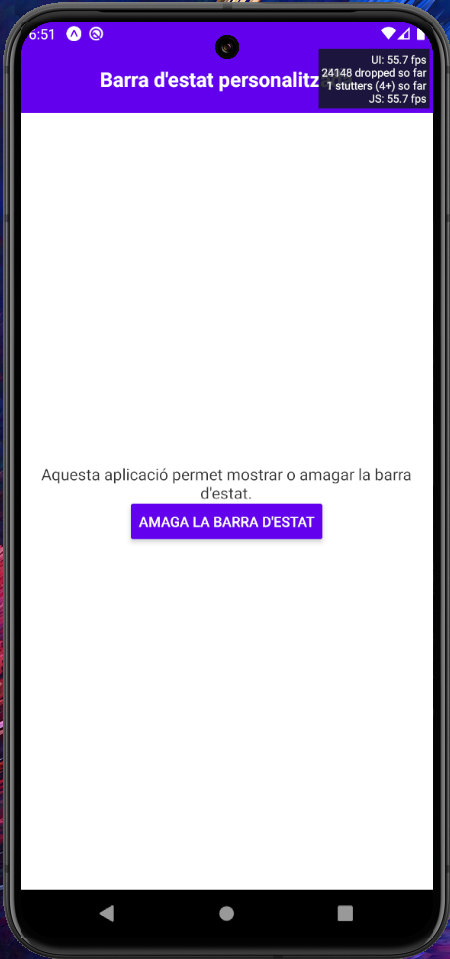
\includegraphics[height=8cm]{ProjectBlank47.png}
		\centering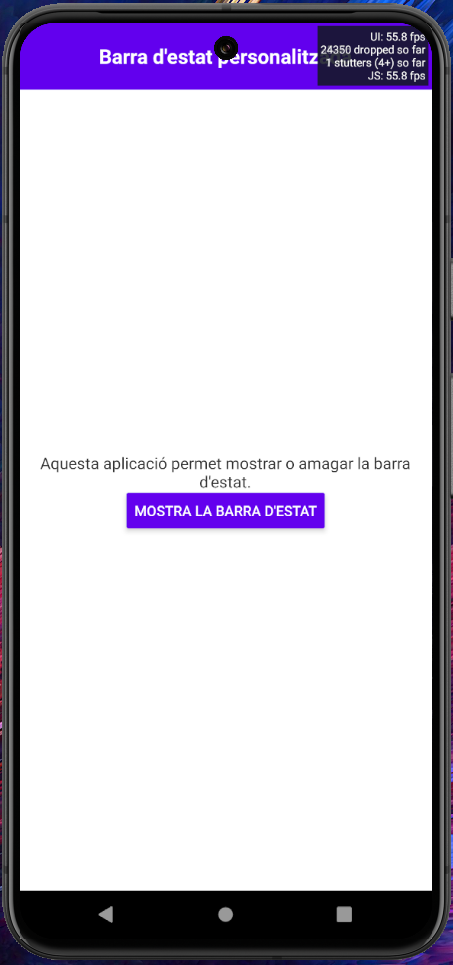
\includegraphics[height=8cm]{ProjectBlank48.png}
	\end{frame}
	\subsubsection{2.2.16. Picker}
	\label{Picker}
	\begin{frame}
		\begin{block}{\texttt{Picker}}
			\texttt{\bf{npm install @react-native-picker/picker}}
			\begin{itemize}
				\item Permet a l'usuari seleccionar un element d'una llista desplegable.
				\item Cada opció es defineix amb un \texttt{Picker.Item}, que té un \texttt{label} (etiqueta visible) i un \texttt{value} (valor intern).
				\item Inclou un \texttt{onValueChange} per gestionar canvis en la selecció.
			\end{itemize}
			Funcionament del següent exemple:
			\begin{itemize}
				\item \texttt{Picker}: Conté les opcions que l'usuari pot seleccionar.
				\item \texttt{Picker.Item}: Defineix cada opció amb etiqueta i valor.
				\item Text de resultat: Mostra el valor seleccionat al \texttt{Picker}.
			\end{itemize}
		\end{block}
	\end{frame}
	\begin{frame}
		\centering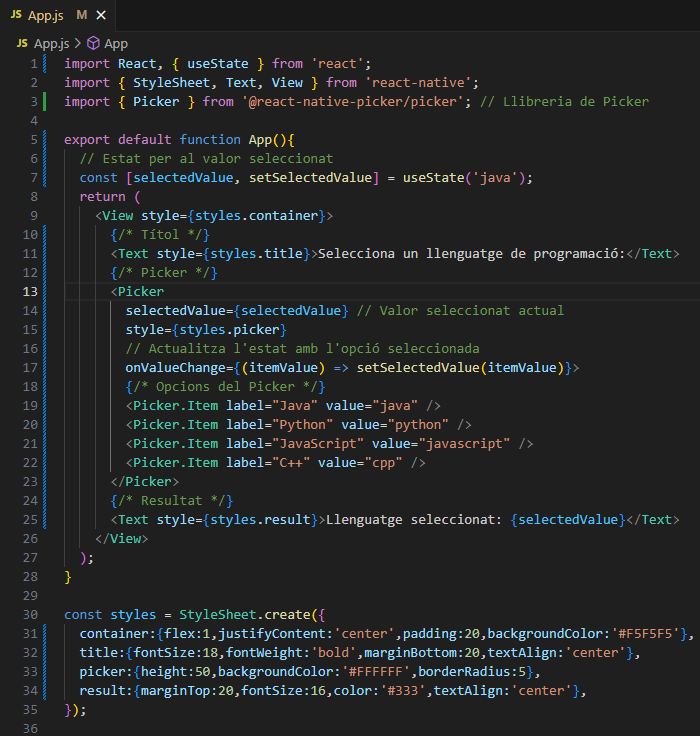
\includegraphics[width=7.5cm]{ProjectBlank49.png}
	\end{frame}
	\begin{frame}
		\centering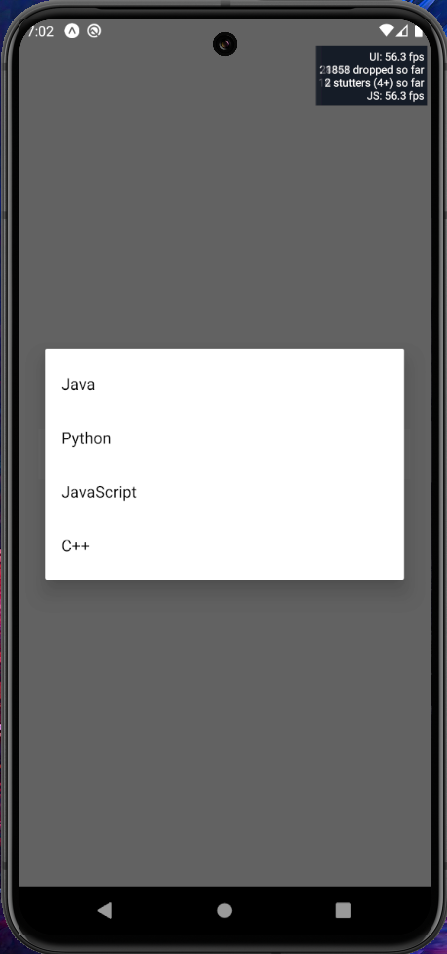
\includegraphics[height=8cm]{ProjectBlank51.png}
		\centering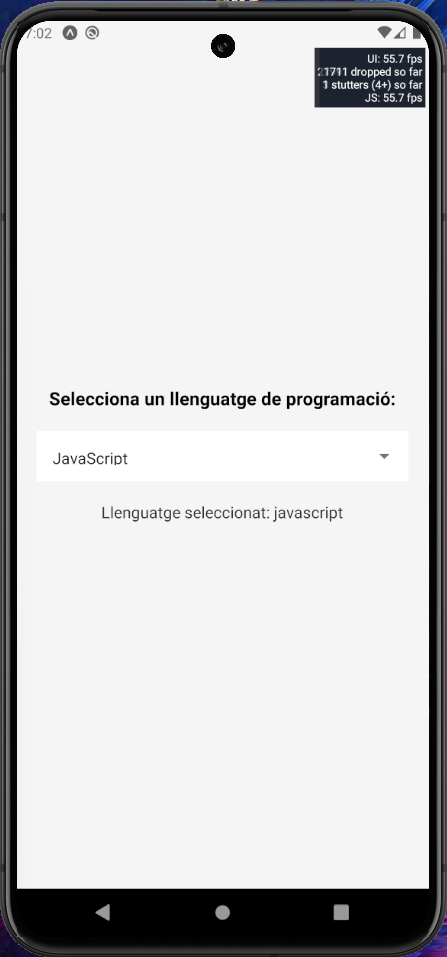
\includegraphics[height=8cm]{ProjectBlank50.png}
	\end{frame}
	\subsubsection{2.2.20. Slider}
	\label{Slider}
	\begin{frame}
	\begin{block}{\texttt{Slider}}
		\texttt{\bf{npm install @react-native-community/slider}}
		\begin{itemize}
			\item Permet ajustar un valor dins d'un rang específic.
			\item Es pot personalitzar amb atributs com \texttt{minimumValue}, \texttt{maximumValue}, \texttt{step}, i colors.
			\item Inclou un \texttt{onValueChange} per gestionar els canvis del valor seleccionat.
		\end{itemize}
		Funcionament del següent exemple:
		\begin{itemize}
			\item \texttt{Slider}: Defineix el rang de valors per a que l'usuari el determini.
			\item \texttt{Text}: Mostra el valor seleccionat per l'usuari.
		\end{itemize}
	\end{block}
	\end{frame}
	
	\begin{frame}
		\centering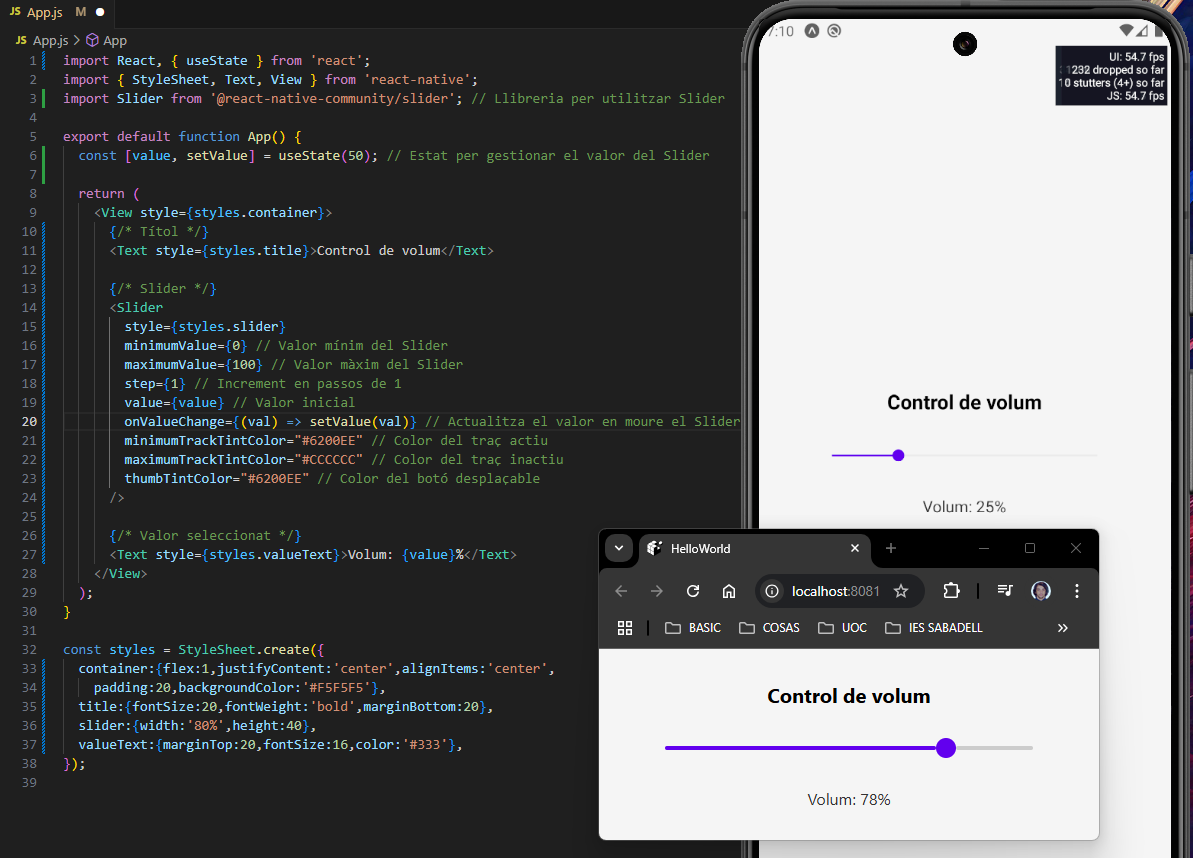
\includegraphics[width=10cm]{ProjectBlank52.png}
	\end{frame}
	\subsubsection{2.2.15. Switch}
	\label{Switch}
	\begin{frame}
		\begin{block}{\texttt{Switch}}
			\begin{itemize}
				\item Component que permet alternar entre dos estats.
				\item Inclou propietats com \texttt{trackColor} per personalitzar el traç i \texttt{thumbColor} per al botó desplaçable.
				\item L'estat es controla amb \texttt{value} i es pot actualitzar amb \texttt{onValueChange}.
			\end{itemize}
			Funcionament del següent exemple:
			\begin{itemize}
				\item \texttt{Switch}: Permet canviar l'estat i personalitzar colors.
				\item Text: Mostra un missatge dinàmic segons l'estat del \texttt{Switch}.
			\end{itemize}
		\end{block}
	\end{frame}
	\begin{frame}
		\centering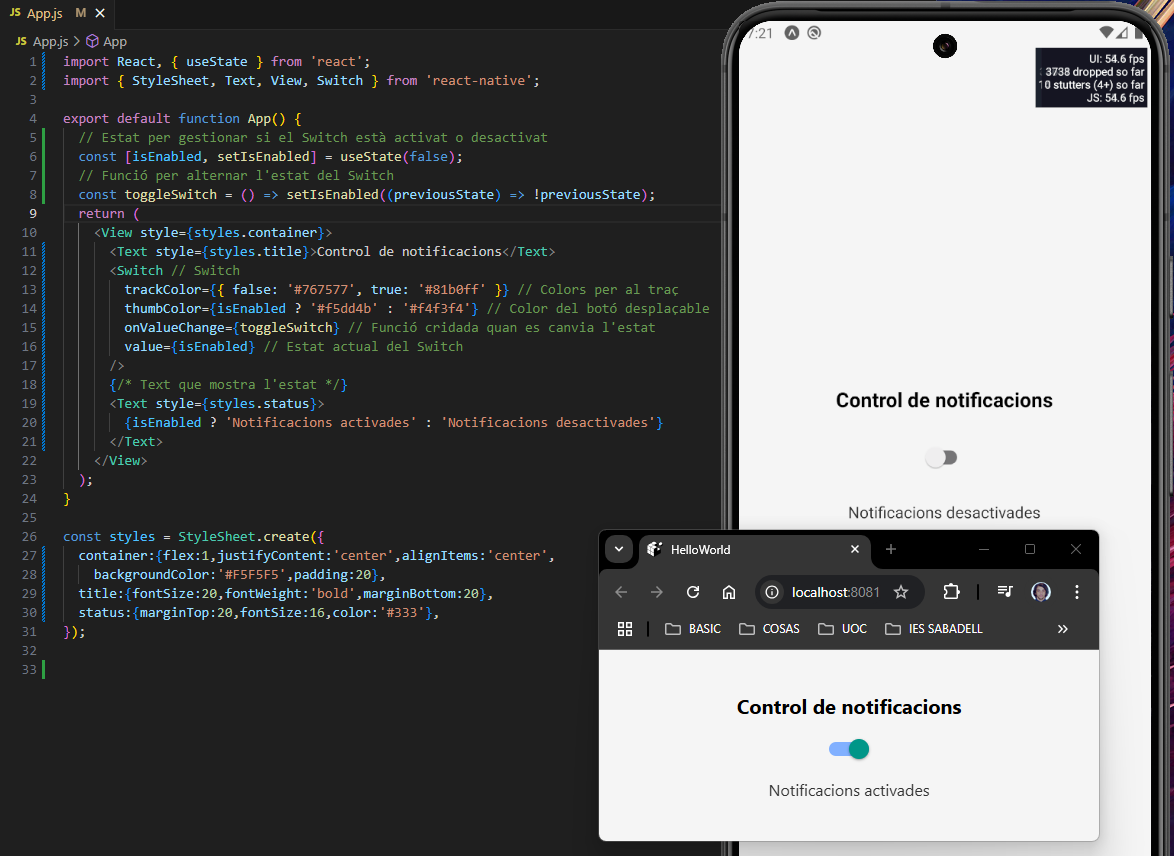
\includegraphics[width=11cm]{ProjectBlank53.png}
	\end{frame}
	\subsection{2.3. Components amb Estils Comuns}
	\subsubsection{2.3.1. Aplicació d'Estils}
	\begin{frame}
		\begin{block}{Ús de \texttt{StyleSheet}}
			\texttt{StyleSheet.create} es una manera optimitzada de crear estils a React Native. Tot i que pots aplicar estils com un objecte JavaScript normal, \texttt{StyleSheet.create} ofereix millors optimitzacions de rendiment.
		\end{block}
		\centering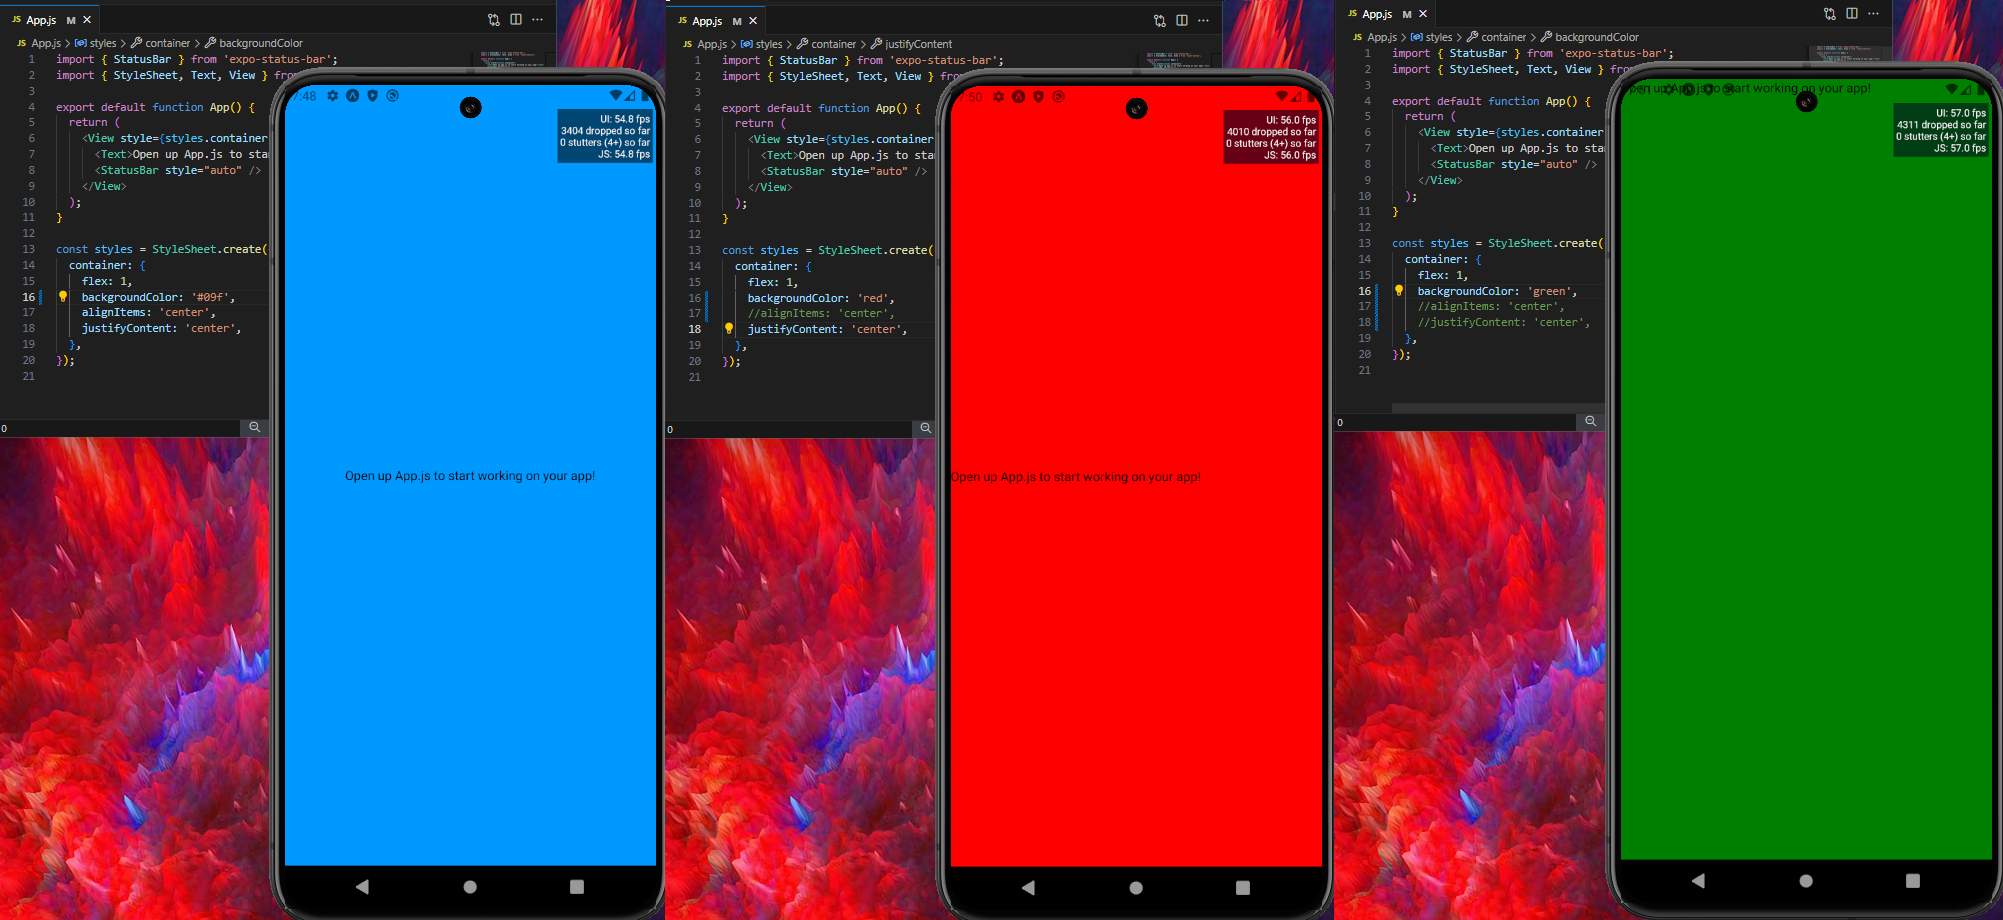
\includegraphics[width=10cm]{ProjectBlank08.png}
	\end{frame}
	\subsubsection{2.3.2. Ús de StyleSheet}
	\begin{frame}
		\centering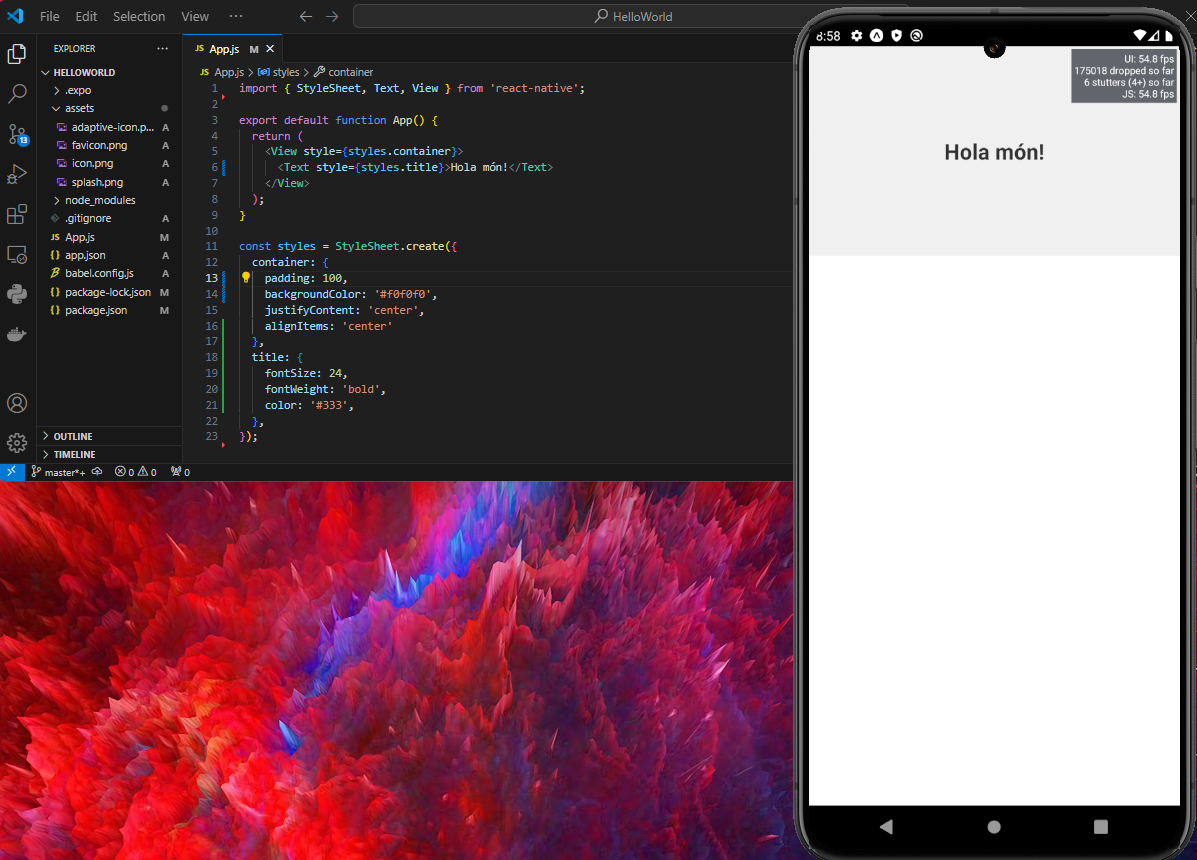
\includegraphics[width=10cm]{ProjectBlank13.png}
	\end{frame}
	\subsubsection{2.3.3. Diferències respecte a CSS}
	\begin{frame}
		\begin{block}{Diferències clau respecte a CSS}
			A React Native, s'utilitzen estils similars als de CSS, però amb algunes diferències:
			
			\begin{enumerate}
				\item CamelCase en comptes de kebab-case\\(e.g., backgroundColor en comptes de background-color).
				\item No s’utilitzen unitats: Els valors numèrics no necessiten px, \%, o altres unitats.
				\item Flexbox per a la distribució dels elements.
				\item No hi ha herència d'estils, cada component té els seus explícits.
			\end{enumerate}
		\end{block}
	\end{frame}
	\subsubsection{2.3.4. Propietats d'Estil Comunes: Dimensions i Colors}
	\begin{frame}
		\begin{block}{Propietats d'Estil Comuns}
			\begin{enumerate}
				\item \textbf{Dimensions} Defineix la mida i disposició dels elements.
					\begin{itemize}
						\item \texttt{width} Amplada del component.
						\item \texttt{height} Alçada del component.
						\item \texttt{maxWidth}/\texttt{maxHeight}/\texttt{minWidth}/\texttt{minHeight} Defineixen la mida màxima/mínima del component.
					\end{itemize}
				\item \textbf{Color i fons}.
					\begin{itemize}
						\item \texttt{backgroundColor} Defineix el color de fons.
						\item \texttt{color} Canvia el color del text en components com \texttt{Text}.
					\end{itemize}
			\end{enumerate}
		\end{block}
	\end{frame}
	\begin{frame}
		\centering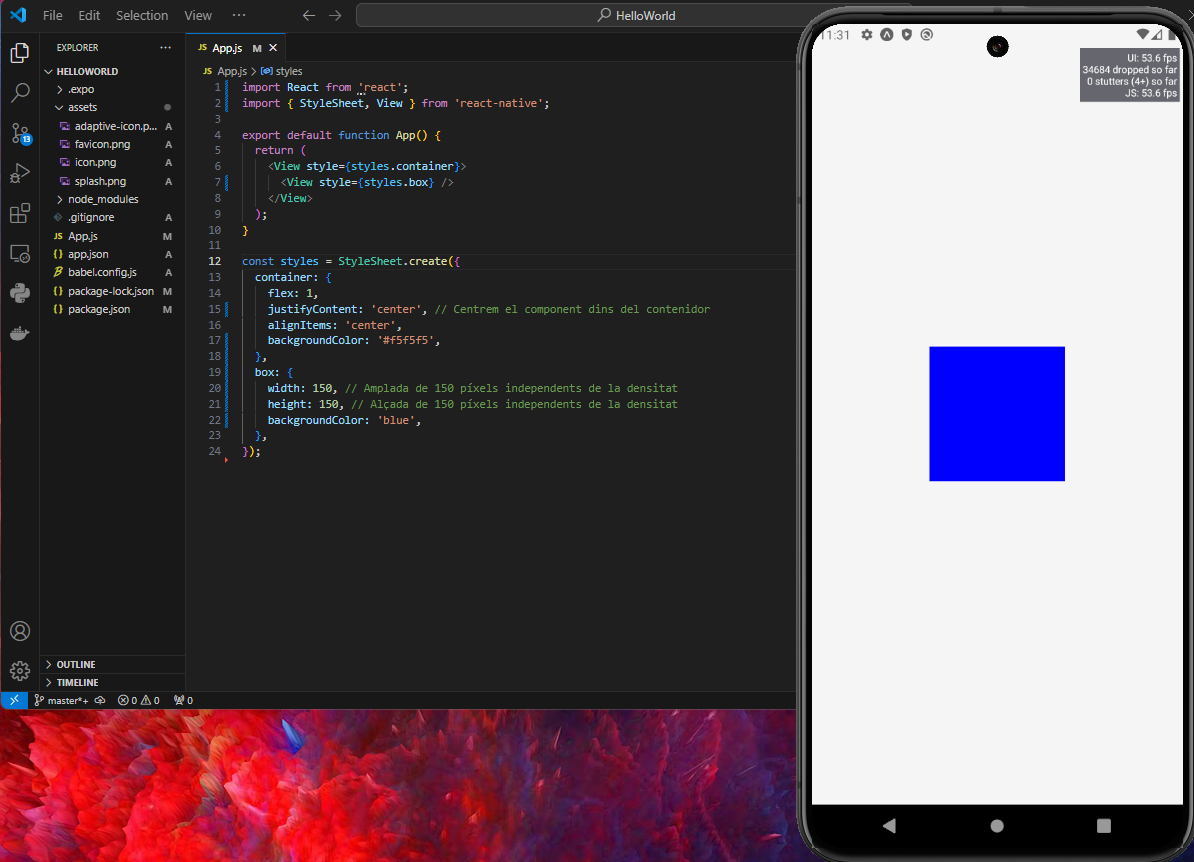
\includegraphics[width=10cm]{ProjectBlank14.png}
	\end{frame}
	\subsubsection{2.3.5. Propietats d'Estil Comunes: Tipografia}
	\begin{frame}
		\begin{block}{Propietats d'Estil Comunes S'HA DE MILLORAR}
			\begin{enumerate}
				\item \textbf{Tipografia}.
				\begin{itemize}
					\item \texttt{fontSize} Mida de la font.
					\item \texttt{fontWeight} Gruix del text(\texttt{normal}, \texttt{bold}, \texttt{100}$-$\texttt{900})
					\item \texttt{textAlign} Alineació del text (\texttt{left}, \texttt{center}, \texttt{right}).
					\item \texttt{lineHeight} Alçada de la línia del text.
					\item \texttt{fontFamily} Defineix la font a utilitzar\\ (com \texttt{Arial}, \texttt{Roboto}, etc).
					\item \texttt{textDecorationLine} Afegeix decoració al text, com ara subratllat o línia a través\\ (\texttt{underline}, \texttt{line-through})
				\end{itemize}
			\end{enumerate}
		\end{block}
	\end{frame}
	\begin{frame}
		\centering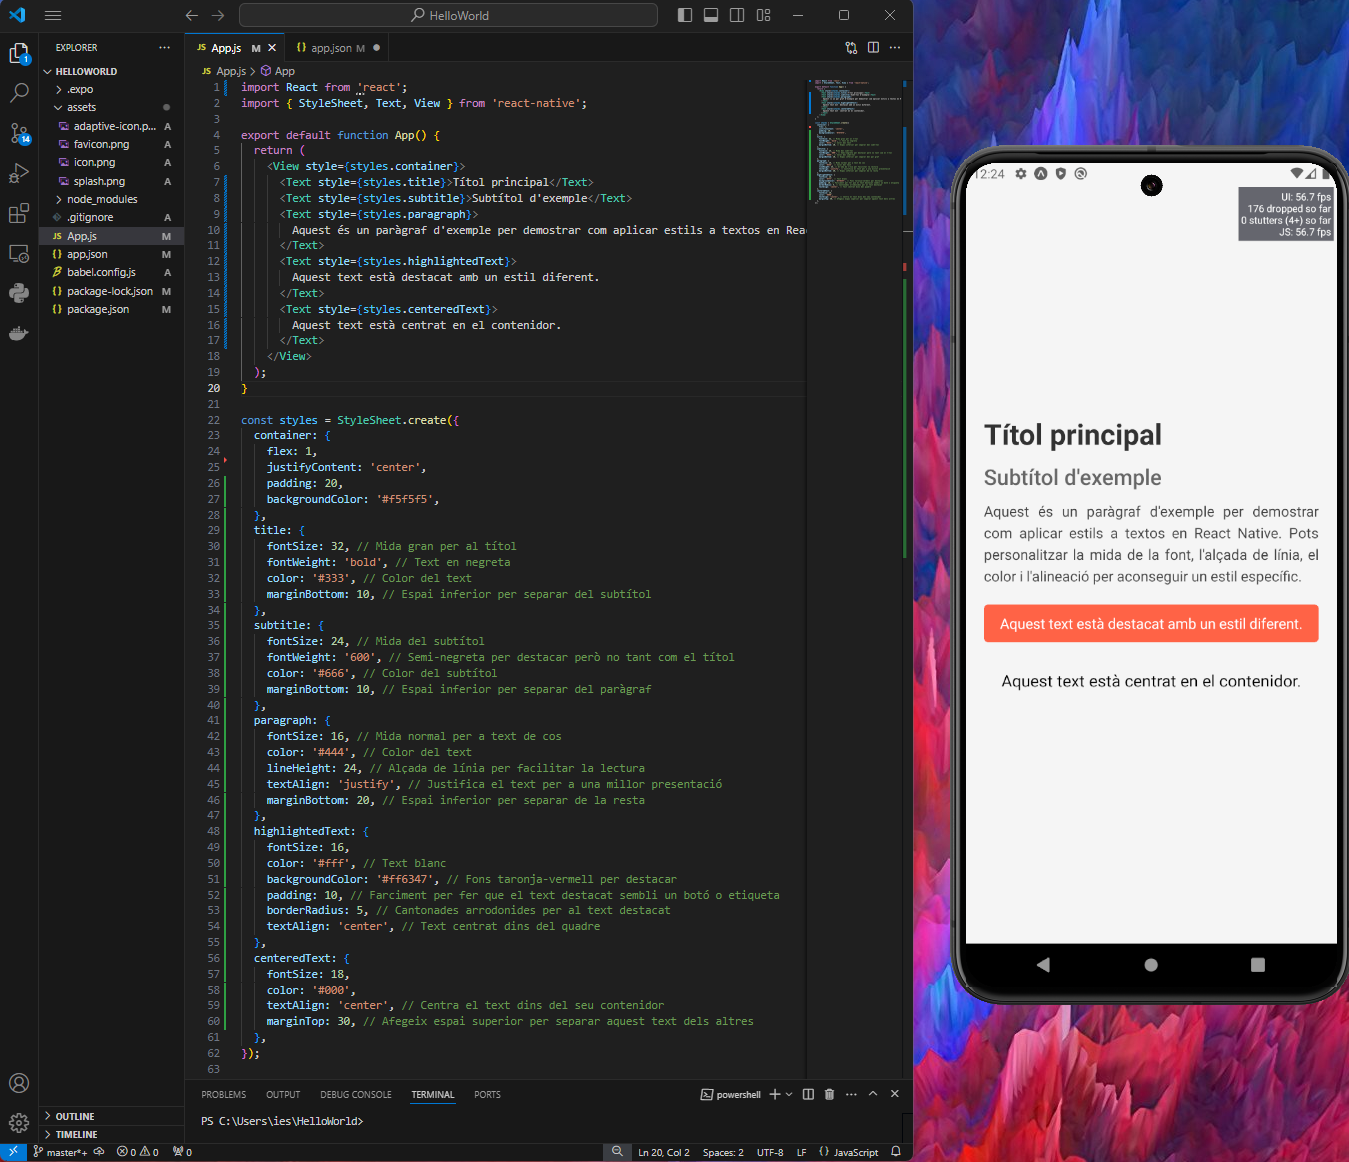
\includegraphics[width=10cm]{ProjectBlank15.png}
	\end{frame}
	\subsubsection{2.3.6. Propietats d'Estil Comunes: Marge i farcit (Spacing)}
	\begin{frame}
		\begin{block}{Propietats d'Estil Comunes}
			\begin{enumerate}
				\item \textbf{Marge i farcit (Spacing)}.
				\begin{itemize}
					\item \texttt{margin} Afegeix espai al voltant d'un component.
					\item \texttt{padding} Afegeix espai dins d'un component, entre el seu contingut i la seva vora.
					\item Valors individuals:
					\begin{itemize}
						\item \texttt{marginTop}, \texttt{marginBottom}, \texttt{marginLeft}, \texttt{marginRight} Ajusta el marge en cada direcció.
						\item \texttt{paddingTop}, \texttt{paddingBottom}, \texttt{paddingLeft}, \texttt{paddingRight} Ajusta el farcit en cada direcció.
					\end{itemize}
				\end{itemize}
			\end{enumerate}
		\end{block}
	\end{frame}
	\begin{frame}
		\centering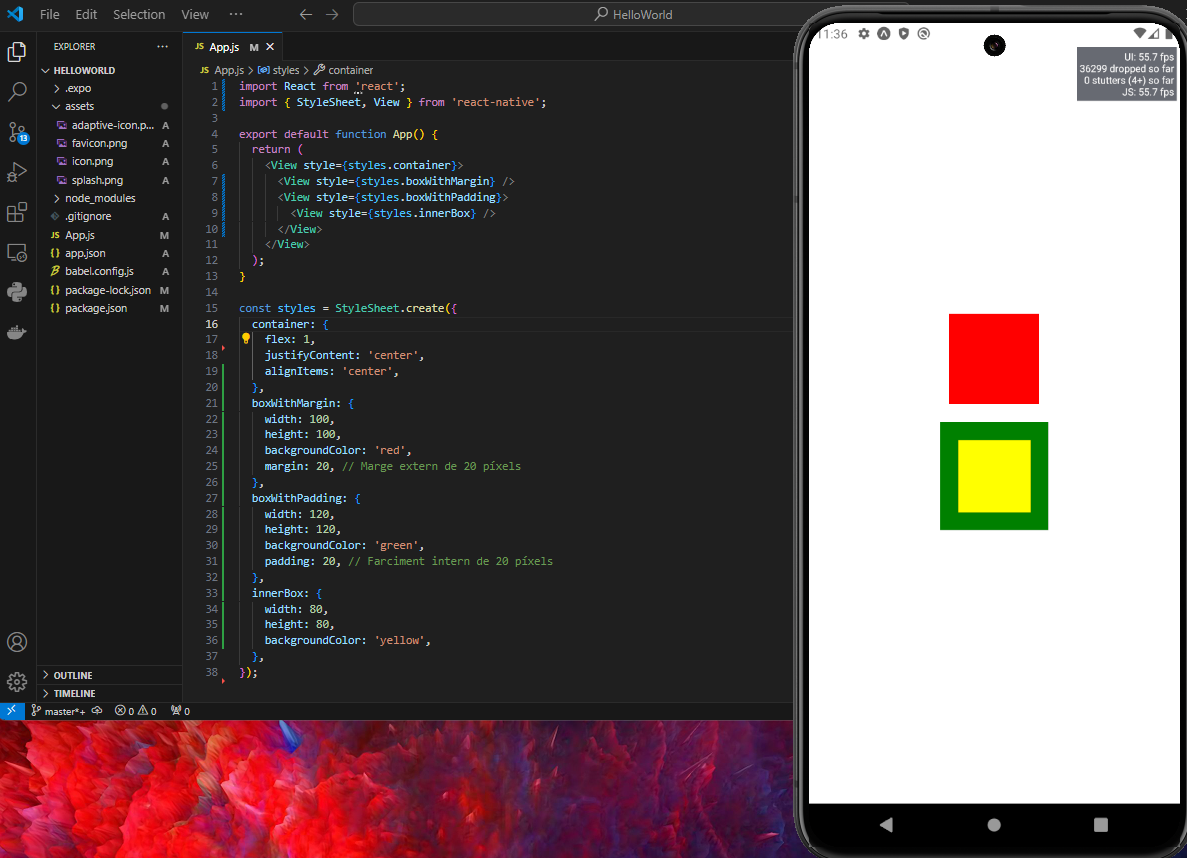
\includegraphics[width=10cm]{ProjectBlank16.png}
	\end{frame}
	\subsubsection{2.3.7. Propietats d'Estil Comunes: Bordes}
	\begin{frame}
		\begin{block}{Propietats 'Estil Comunes}
			\begin{enumerate}
				\item \textbf{Bordes}.
				\begin{itemize}
					\item \texttt{borderWidth} Gruix de la vora.
					\item \texttt{borderColor} Color de la vora.
					\item \texttt{borderRadius} Crea vores arrodonides
				\end{itemize}
			\end{enumerate}
		\end{block}
	\end{frame}
	\begin{frame}
		\centering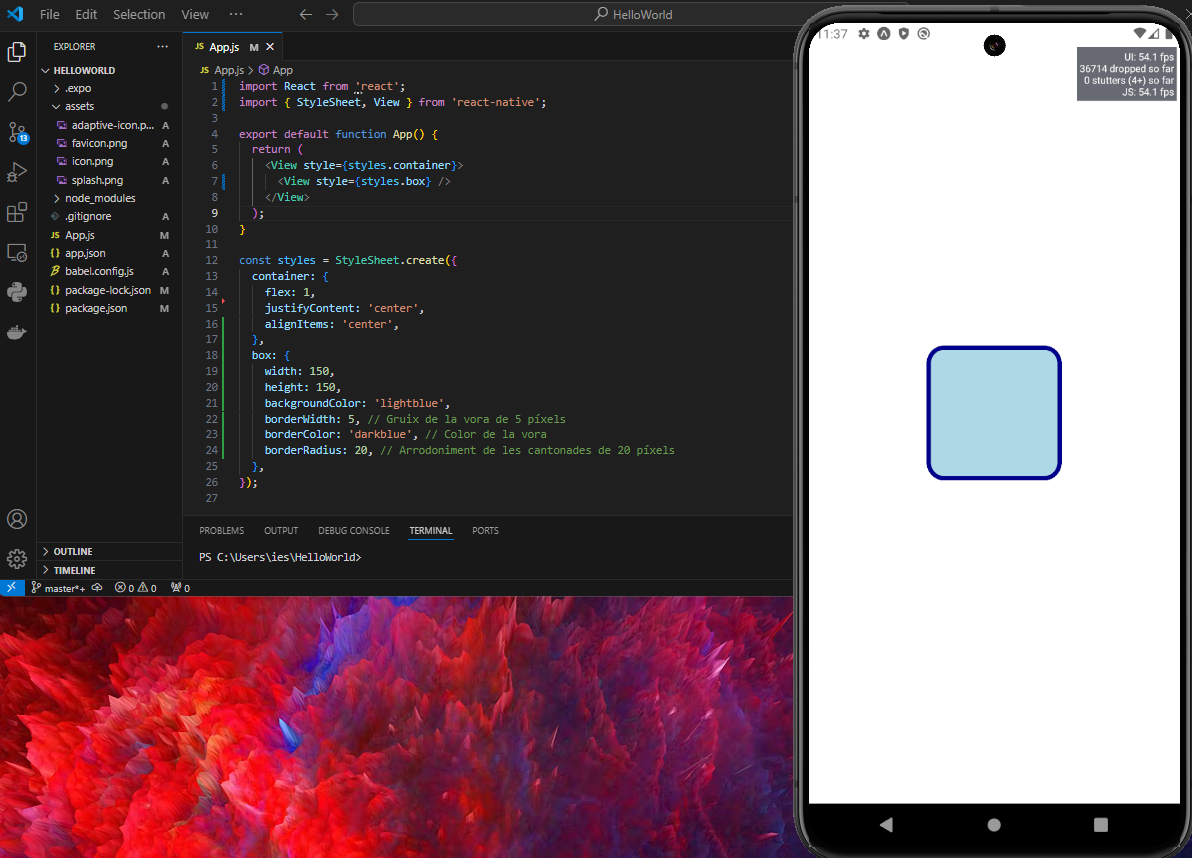
\includegraphics[width=10cm]{ProjectBlank17.png}
	\end{frame}
	\subsection{2.4. Components Flexbox}
	\subsubsection{2.4.0. Teoria dels components Flexbox}
	\begin{frame}
		\begin{block}{Flex, Components Flexbox}
			El sistema de disseny flexible basat en Flexbox, \textbf{Flex} es una eina molt poderosa per crear interfícies d'usuari adaptables i distribuïdes de manera eficient en diferents mides de pantalla.
		\end{block}
	\end{frame}
	\subsubsection{2.4.1. FlexDirection}
	\begin{frame}
		\begin{block}{Conceptes Clau de Flexbox a React Native}
			\texttt{\bf{flexDirection}} Defineix la direcció en què es distribueixen els elements fills dins d'un contenidor. Els valors més comuns són:
			\begin{itemize}
				\item \texttt{row} Col$\cdot$loca els elements horitzontalment.
				\item \texttt{column} Col$\cdot$loca els elements verticalment.
			\end{itemize}
		\end{block}
	\end{frame}
	\begin{frame}
		\centering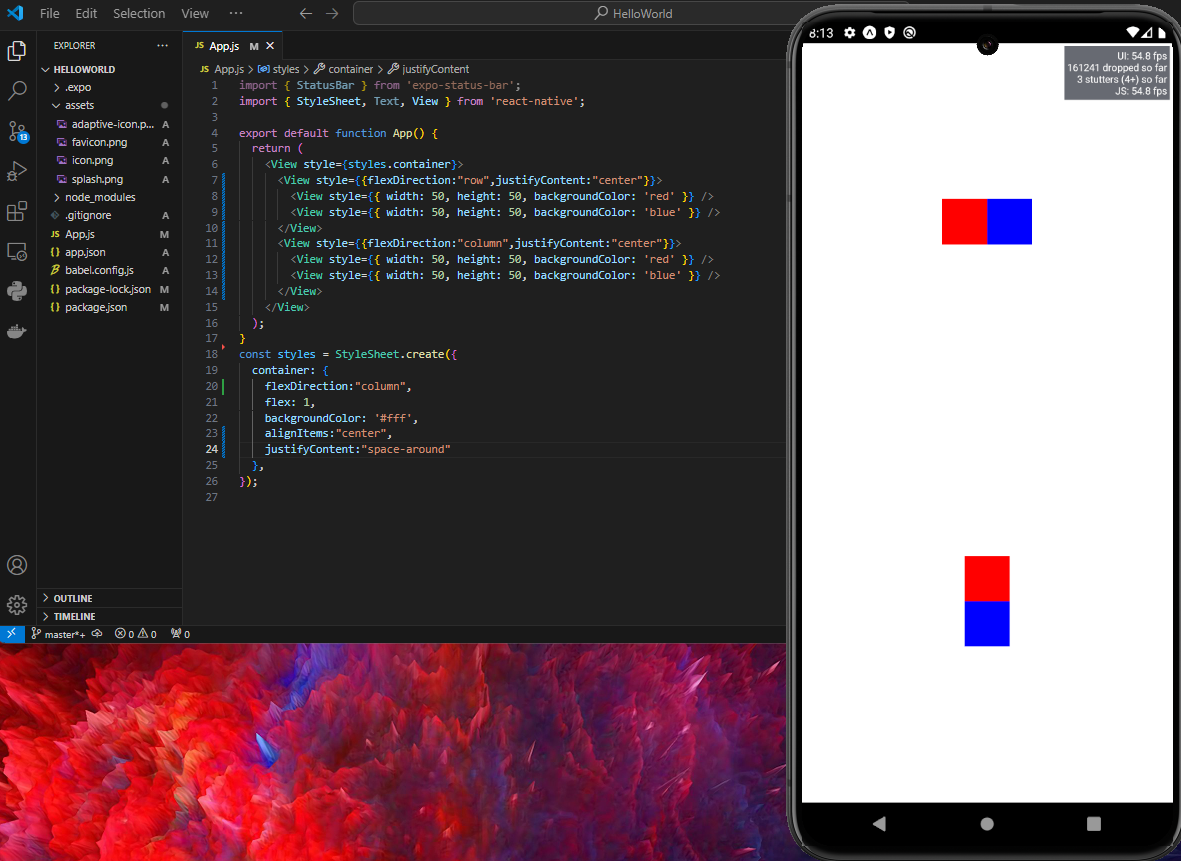
\includegraphics[width=10cm]{ProjectBlank09.png}		
	\end{frame}
	\subsubsection{2.4.2. Flex}
	\begin{frame}
		\begin{block}{Conceptes Clau de Flexbox a React Native}
			\texttt{\bf{Flex}} Estableix quant d'espai ha d'ocupar un element dins del seu contenidor pare, d'acord amb l'espai disponible.\\
			Si diversos elements tenen un valor de flex, l'espai disponible es dividirà proporcionalment entre ells.
			\begin{itemize}
				\item Un valor més gran de \texttt{flex} significa que aquest element ocuparà més espai relatiu.
				\item Si no s'especifica \texttt{flex}, l'element ocuparà només la mida del seu contingut.
			\end{itemize}
		\end{block}
	\end{frame}
	\begin{frame}
		\centering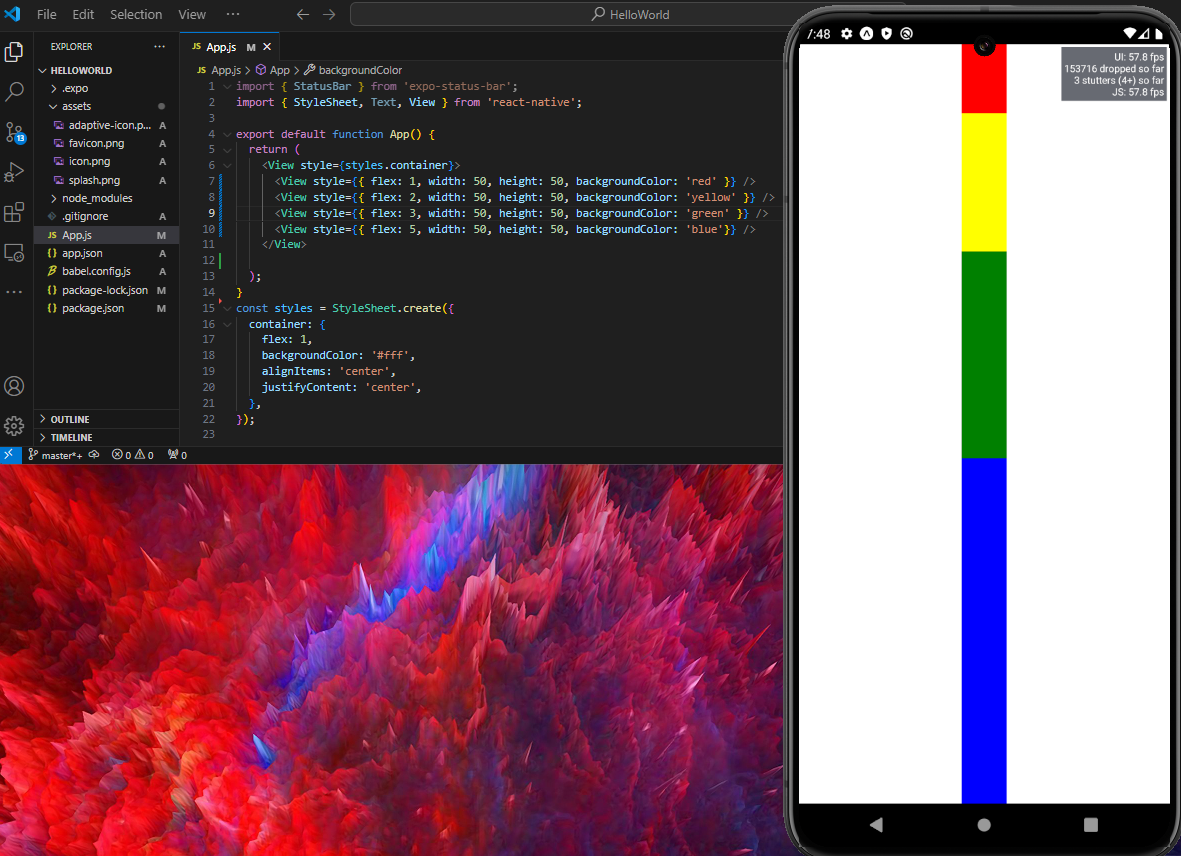
\includegraphics[width=10cm]{ProjectBlank10.png}
	\end{frame}
	\subsubsection{2.4.3. JustifyContent}
	\begin{frame}
		\begin{block}{Conceptes Clau de Flexbox a React Native}
			\texttt{\bf{justifyContent}} Defineix com es distribueixen els elements al llarg de l'eix principal (el definit per\texttt{flexDirection}). Valors comuns:
			\begin{itemize}
				\item \texttt{flex-start} Alinea els elements al principi de l'eix.
				\item \texttt{center} Alinea els elements al centre.
				\item \texttt{flex-end} Alinea els elements al final.
				\item \texttt{space-between} Distribueix els elements amb el màxim espai possible entre ells.
				\item \texttt{space-around} Distribueix els elements amb un espai igual al voltant de cada una.
			\end{itemize}
		\end{block}
	\end{frame}
	\begin{frame}
		\centering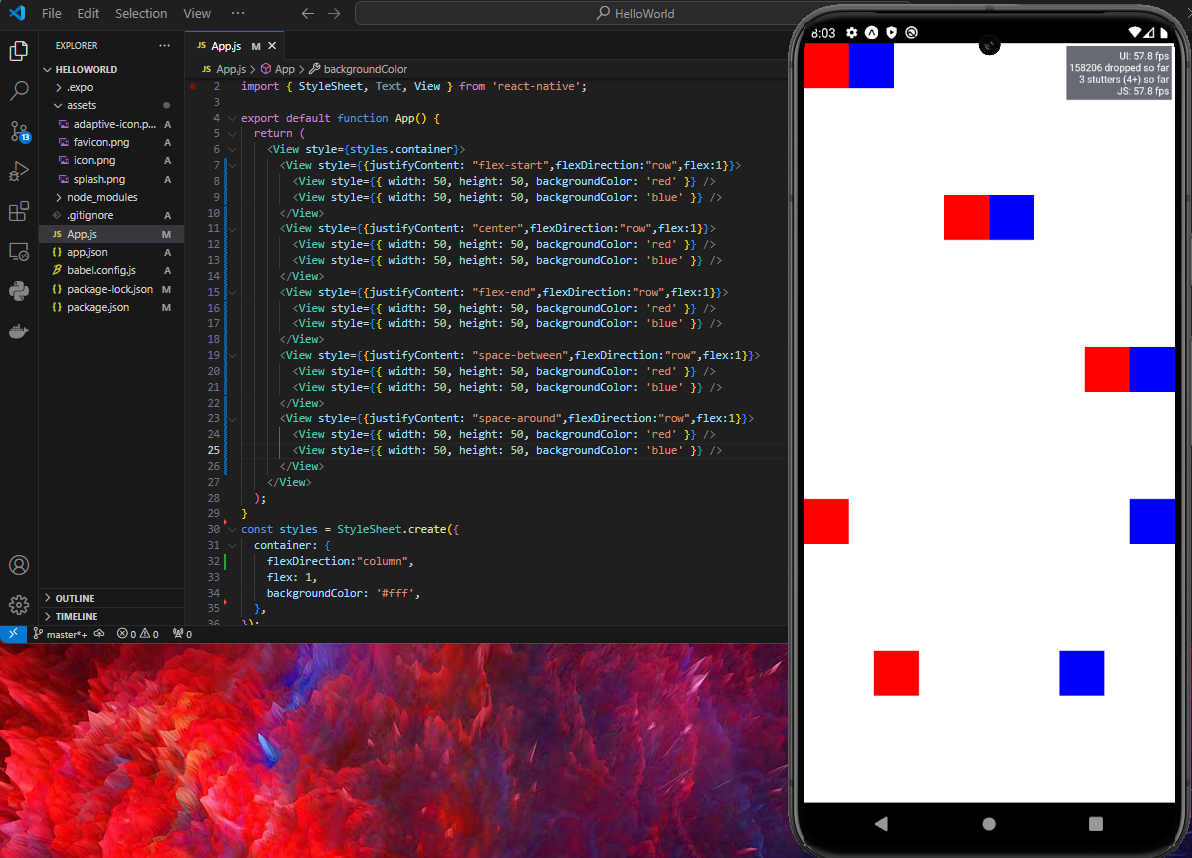
\includegraphics[width=10cm]{ProjectBlank11.png}
	\end{frame}
	\subsubsection{2.4.4. AlignItems}
	\begin{frame}
		\begin{block}{Conceptes Clau de Flexbox a React Native}
			\texttt{\bf{alignItems}} Controla com s'alineen els elements al llarg de l'eix secundari (perpendicular al definit per \texttt{flexDirection}).Valors comuns:
			\begin{itemize}
				\item \texttt{flex-start} Alinea els elements al principi de l'eix secundari.
				\item \texttt{center} Alinea els elements al centre de l'eix secundari.
				\item \texttt{flex-end} Alinea els elements al final.
				\item \texttt{stretch} Estira els elements perquè omplia tot l'espai disponible a l'eix secundari.
			\end{itemize}
		\end{block}
	\end{frame}
	\begin{frame}
		\centering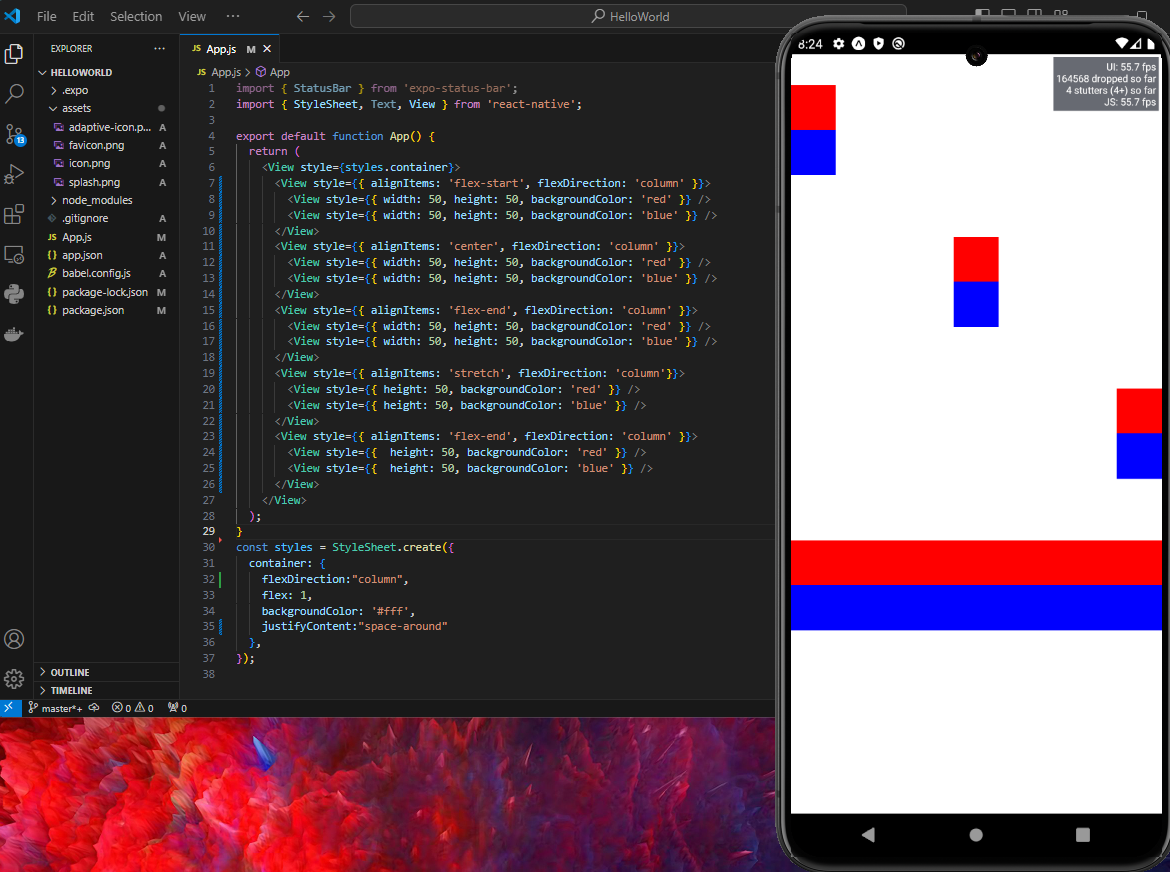
\includegraphics[width=10cm]{ProjectBlank12.png}
	\end{frame}
	\section{3. Complexitat de les Possibilitats d'Estils}
	\subsection{3.1. Combinació d'Estils}
	\subsubsection{3.1.1. Combinació d'Estils}
	\begin{frame}
		\begin{block}{Combinació d'Estils}
			React Native permet combinar múltiples objectes d'estil en un mateix component. Això és útil quan vols aplicar diversos estils que poden estar separats lògicament però que es poden fusionar quan s'apliquen a un mateix element.\\
		\end{block}
		\begin{block}{}
			Per aplicar diversos estils a un component, podem utilitzar una matriu a la propietat \texttt{style}
		\end{block}
	\end{frame}
	\begin{frame}
		\centering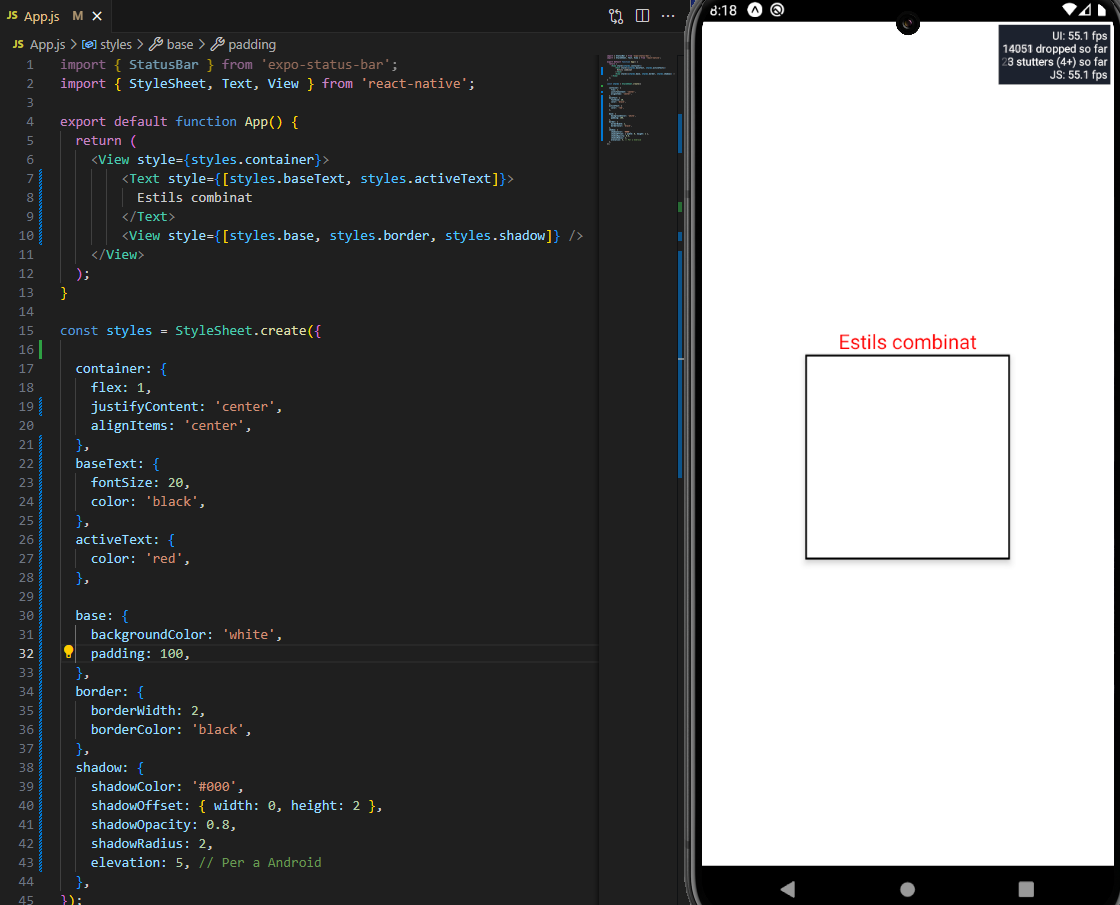
\includegraphics[width=10cm]{ProjectBlank18.png}
	\end{frame}
	\subsection{3.2. Estils per a Plataformes Específiques}
	\subsubsection{3.2.1. Platform.select()}
	\begin{frame}
		\begin{block}{}
			A React Native es pot crear estils específics per a cada plataforma (iOS, Android, Web, etc) amb l'objecte \texttt{Platform}, útil per aplicar estils diferents a causa de diferències de disseny o comportament entre les plataformes.
		\end{block}
		\begin{block}{Ús de \texttt{Platform.select()}}
				\texttt{Platform.select()} et permet definir estils diferents per a cada plataforma en un mateix bloc de codi. Accepta un objecte amb clau de plataforma \texttt{ios}, \texttt{android} i \texttt{web}.
		\end{block}
		\begin{block}{\texttt{Platform.OS} i \texttt{Platform.Version}}
		Es pots fer ús de \texttt{Platform.OS} per aplicar condicionalment certs estils dins del component i amb \texttt{Platform.Version} es pot accedir a la versió específica del sistema operatiu i fer condicions basades en ella.
		\end{block}
	\end{frame}
	\begin{frame}
		\centering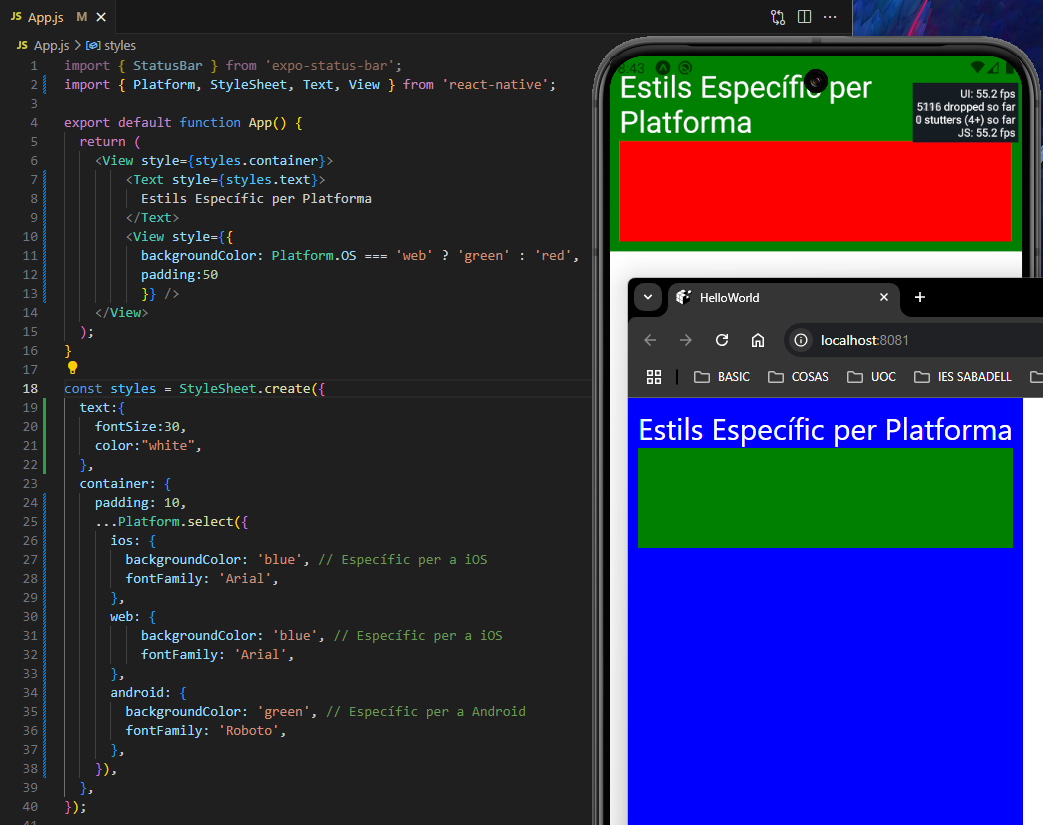
\includegraphics[width=10cm]{ProjectBlank19.png}
	\end{frame}
	\subsection{3.3. Estils Dinàmics segons Estats}
	\subsubsection{3.3.1. Estils segons estat}
	\begin{frame}
		\begin{block}{Canviar l'estil segons l'estat \texttt{useState}}
			Es pot utilitzar una variable d'estat (isActive) per canviar l'estil del text i el color de fons d'un botó.
		\end{block}
		\centering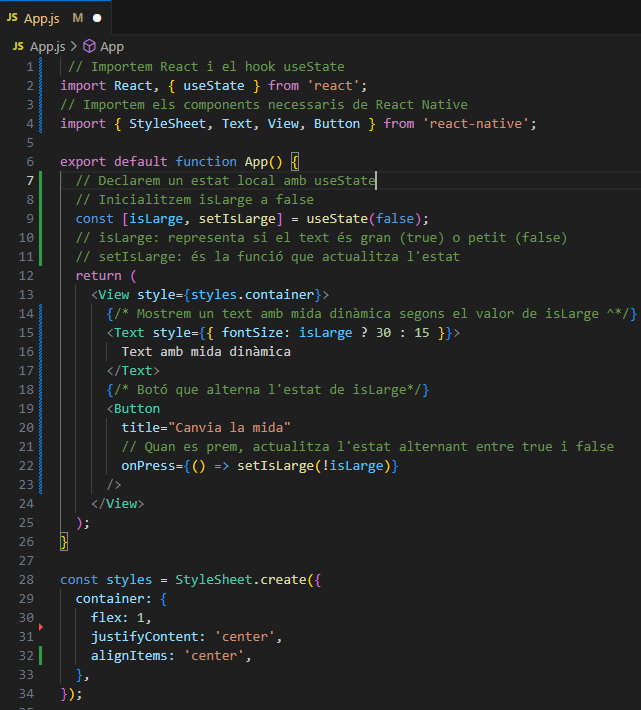
\includegraphics[height=5.5cm]{ProjectBlank20.png}
		\centering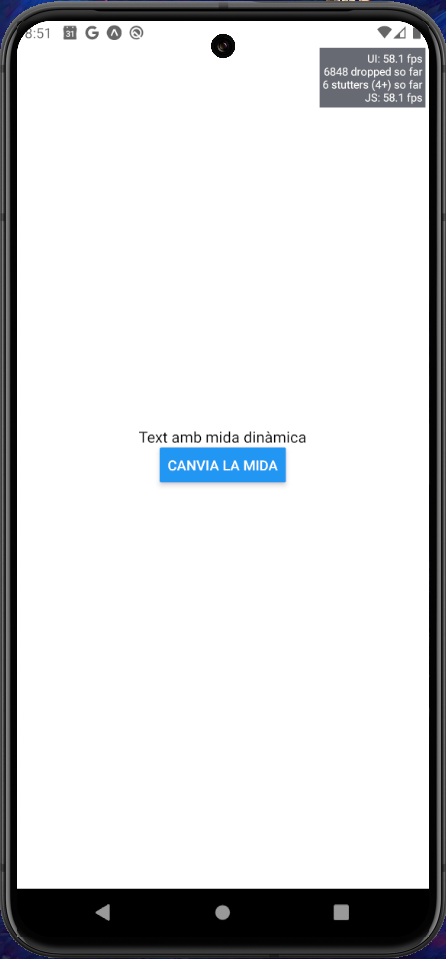
\includegraphics[height=5.5cm]{ProjectBlank21.png}
		\centering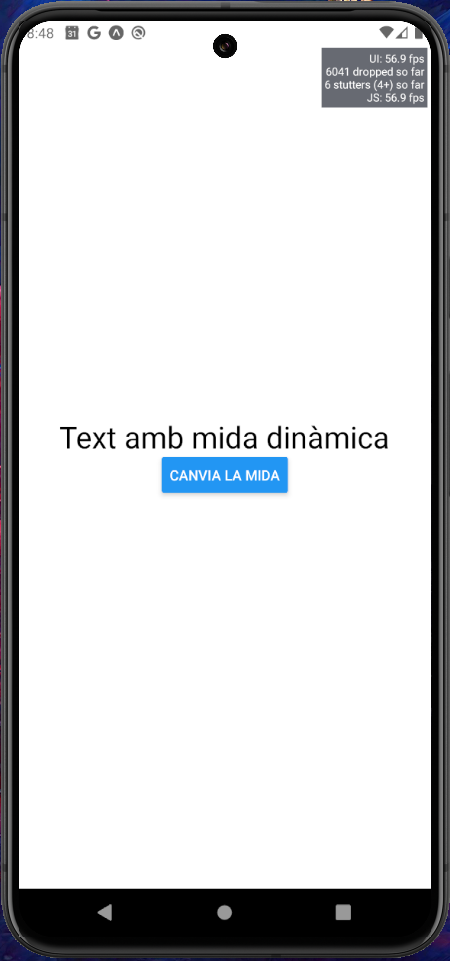
\includegraphics[height=5.5cm]{ProjectBlank22.png}
	\end{frame}
	\begin{frame}
		\centering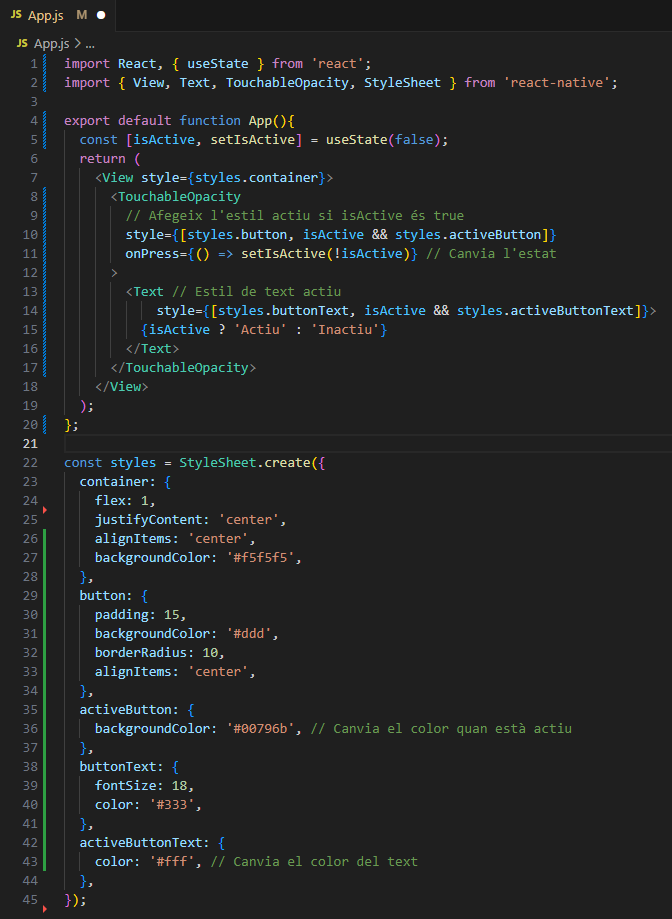
\includegraphics[height=5.5cm]{ProjectBlank23.png}
		\centering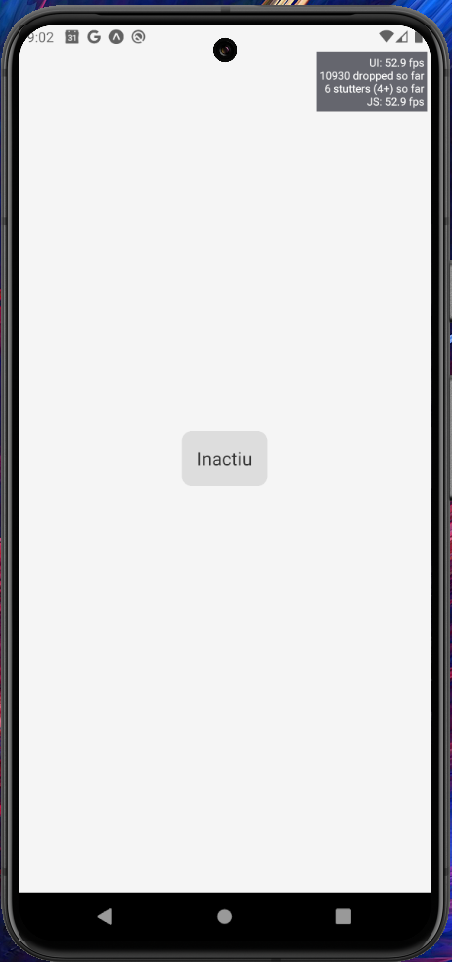
\includegraphics[height=5.5cm]{ProjectBlank24.png}
		\centering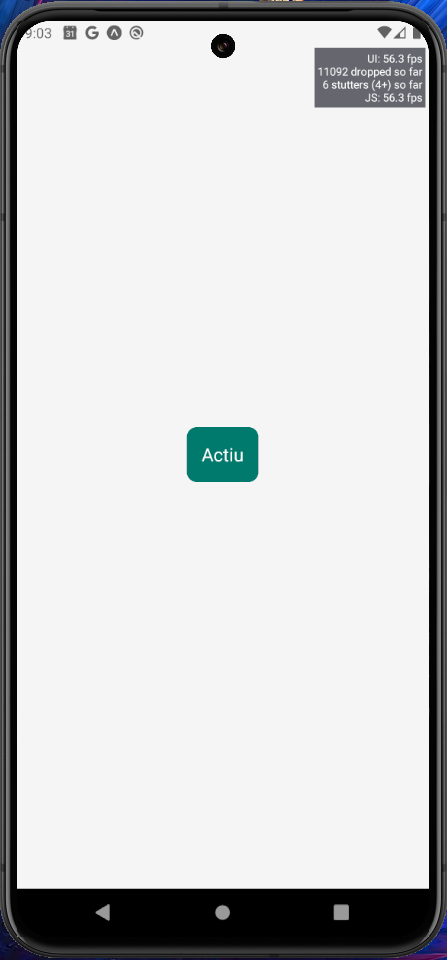
\includegraphics[height=5.5cm]{ProjectBlank25.png}
	\end{frame}
	\subsection{3.4. Estils Dinàmics Funcionals i Condicionals}
	\subsubsection{3.4.1. Estil funcionals}
	\begin{frame}
		\begin{block}{Funcions d'Estils i Estils Condicionals}
			Es poden fer funció per generar estils segons valors.\\
			També fer condicions als diccionaris d'estils.
		\end{block}
		\centering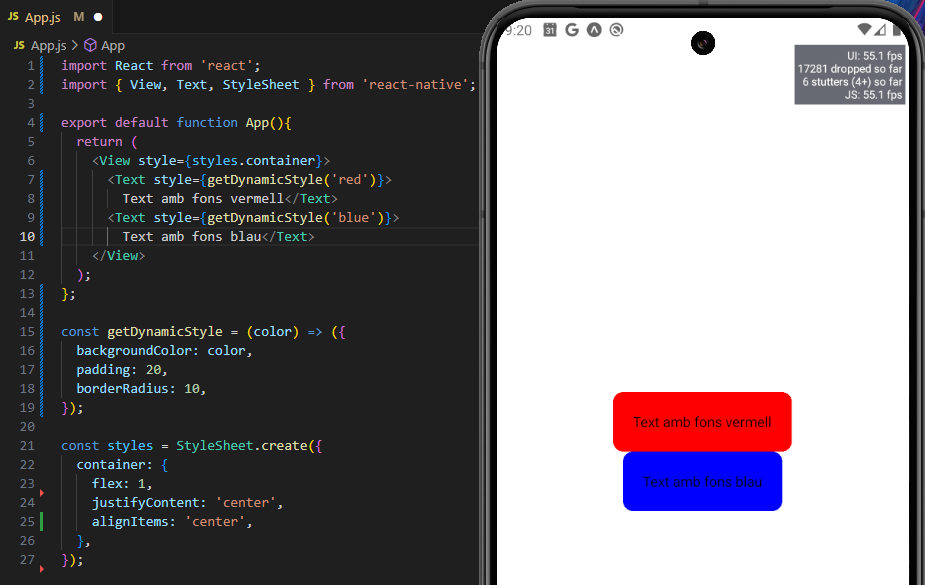
\includegraphics[width=9cm]{ProjectBlank27.png}
	\end{frame}
	\subsubsection{3.4.2. Estil condicionals}
	\begin{frame}
		\centering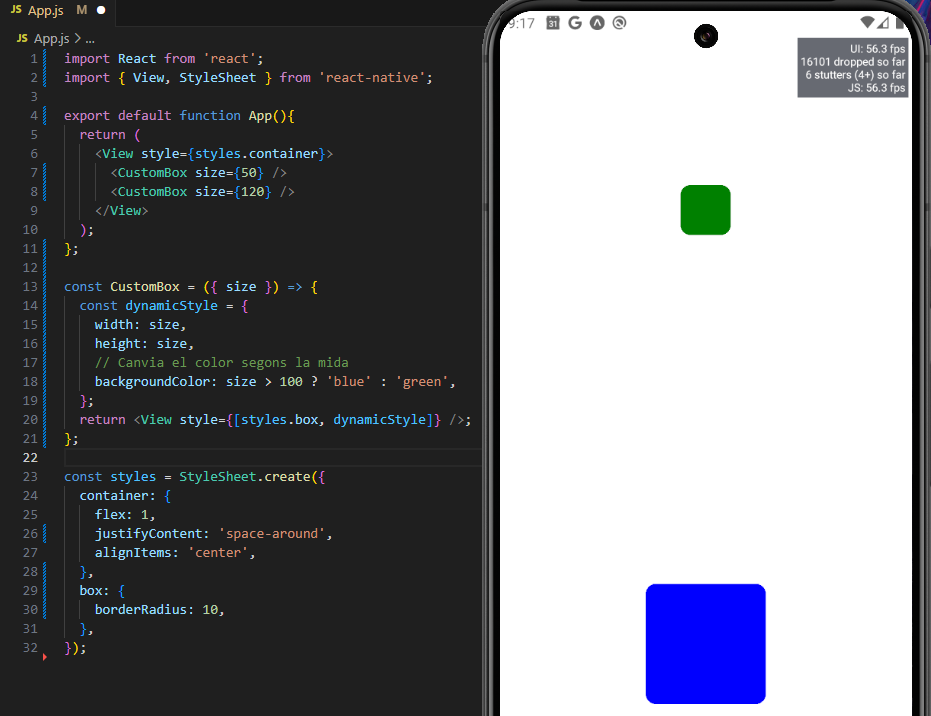
\includegraphics[width=9cm]{ProjectBlank26.png}
	\end{frame}
	\subsection{3.4. Estils Dinàmics Animats}
	\subsubsection{3.4.1. Estils Animats}
	\begin{frame}
		\begin{block}{Estils animats amb \texttt{Animated.timing}}
			Combinem animacions i estils dinàmics amb \texttt{Animated}.
		\end{block}
		\centering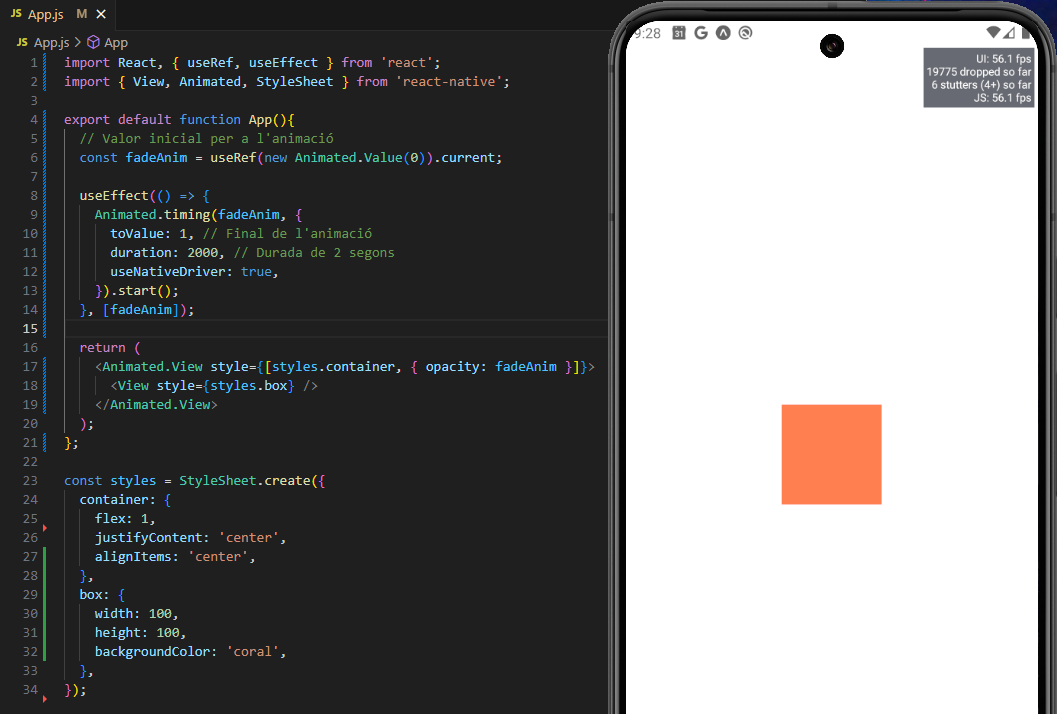
\includegraphics[width=9cm]{ProjectBlank28.png}
	\end{frame}
	\subsubsection{3.4.2. Estils Animats Oscilanció}
	\begin{frame}
		\begin{block}{\texttt{Animated.loop} i \texttt{Animated.sequence}}
			Amb aquestes funcions podem elaborar més les animacions.
		\end{block}
		\centering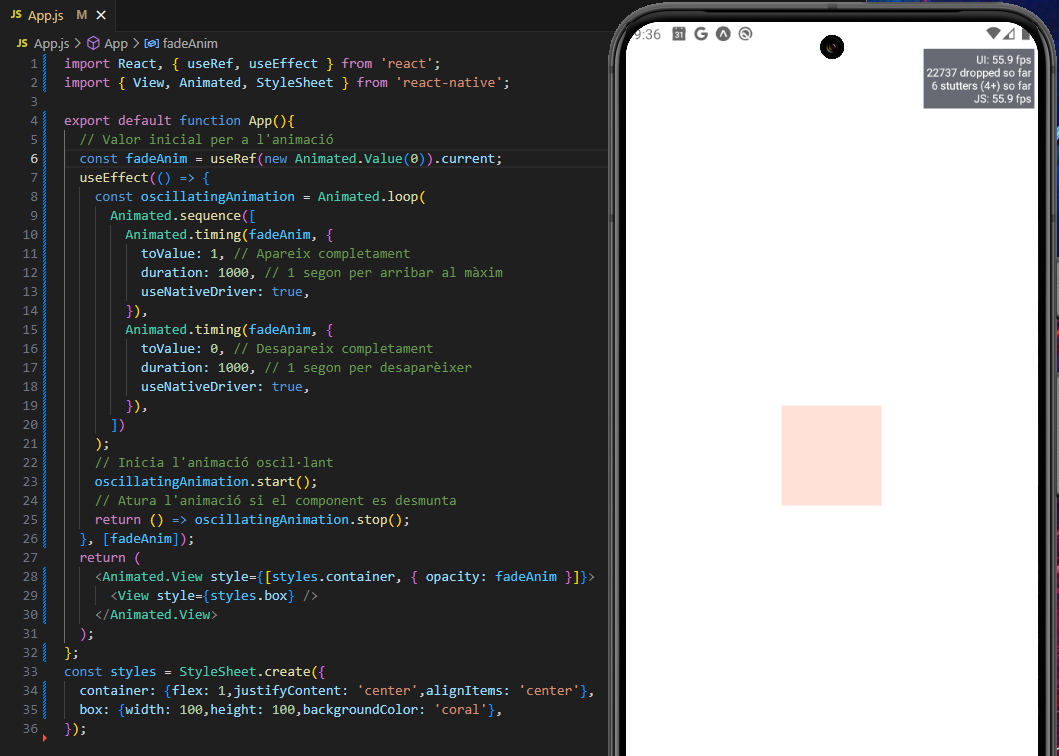
\includegraphics[width=9cm]{ProjectBlank29.png}
	\end{frame}
	\section{4. Navegació a React Native}
	\subsection{4.1. React Navigation: Introducció}
	\subsubsection{4.1.0. Introducció}
	\begin{frame}
		\begin{block}{Introducció a React Navigation}
			React Navigation és una de les llibreries més utilitzades per gestionar navegació a React Native.
		\end{block}
		\begin{block}{}
			Ofereix diverses opcions de navegació, com navegació en pila, pestanyes, menús laterals, i navegació basada en profunditat (nested navigation). Aquesta subsecció explica com instal·lar i configurar React Navigation en un projecte.
		\end{block}
	\end{frame}
	\subsubsection{4.1.1. Configuració de React Navigation}
	\begin{frame}
		\begin{block}{Instal$\cdot$lació de dependències bàsiques}
			\centering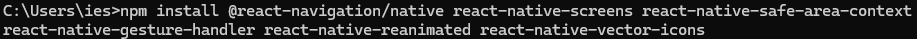
\includegraphics[width=10cm]{Continua01.png}\\
			\raggedright Aquestes dependències inclouen:
			\begin{enumerate}
				\item \texttt{react-navigation/native}: Nucli de la navegació.
				\item \texttt{react-native-screens}: Renderització de pantalles.
				\item \texttt{react-native-safe-area-context}: Zones segures.
				\item \texttt{react-native-gesture-handler}: Gestos tàctils.
				\item \texttt{react-native-reanimated}: Animacions avançades.
				\item \texttt{react-native-vector-icons}: Icones per a navegació.
			\end{enumerate}			
		\end{block}
	\end{frame}
	\subsubsection{4.1.2. Tipus de Navegació}
	\begin{frame}
		\begin{block}{Tipus de Navegacions de React Navigation}
			React Navigation és molt versàtil permetent gestionar diversos tipus de navegació. Ofereix:
			\begin{itemize}
				\item Stack Navigator: Navegació jeràrquica de pila d'ecrans.\\
					\texttt{npm install @react-navigation/native-stack}
				\item Tab Navigator: Navegació per pestanyes independents.\\
					\texttt{npm install @react-navigation/bottom-tabs}
				\item Drawer Navigator: Un menú lateral desplegable per accedir a diferents funcionalitats.\\
					\texttt{npm install @react-navigation/drawer}
			\end{itemize}
		\end{block}
	\end{frame}
	\subsubsection{4.1.3. Configuració del react-native-reanimated}
	\begin{frame}
		\begin{block}{Configuració de \texttt{react-native-reanimated}}
			\texttt{\bf{npm install --save-dev metro-react-native-babel-preset}}\\
			Afegiu el plugin necessari per a \texttt{react-native-reanimated} i
			 reinicieu el projecte expo amb \texttt{npm start --reset-cache}.
		\end{block}
		\centering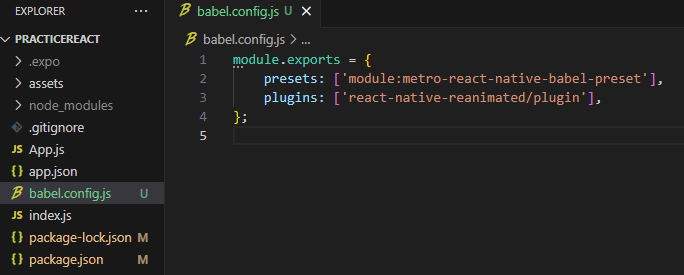
\includegraphics[width=11cm]{Continua02.png}
	\end{frame}
	\subsection{4.2. React Navigation: Stack Navigator}
	\subsubsection{4.2.1. Stack Navigator}
	\begin{frame}
		contenidos...
	\end{frame}
	\subsection{4.3. React Navigation: Tab Navigator}
	\subsubsection{4.1.3. Tab Navigator}
	\begin{frame}
		contenidos...
	\end{frame}
	\subsection{4.4. React Navigation: Drawer Navigator}
	\subsubsection{4.1.4. Drawer Navigator}
	\begin{frame}
		contenidos...
	\end{frame}
	\subsection{4.2. Navegació entre Pantalles}
	\subsubsection{4.2.1. Passar Paràmetres entre Pantalles}
	\subsubsection{4.2.2. Tornar a Pantalles Anteriors (Go Back)}
	\subsubsection{4.2.3. Control de l'Estat de Navegació}
	
	\section{5. Gestió d'Estat}
	
	\subsection{5.1. Gestió Bàsica amb \texttt{useState} i \texttt{useReducer}}
	\subsubsection{5.1.1. Estat Local amb \texttt{useState}}
	\subsubsection{5.1.2. Flux Complex amb \texttt{useReducer}}
	
	\subsection{5.2. Gestió Avançada amb Context API}
	\subsubsection{5.2.1. Creació de Context}
	\subsubsection{5.2.2. Consumir Context als Components}
	
	\subsection{5.3. Llibreries de Gestió d'Estat}
	\subsubsection{5.3.1. Redux Toolkit}
	\subsubsection{5.3.2. Zustand o Recoil}
	
	\section{6. Connexió amb APIs i Bases de Dades}
	
	\subsection{6.1. Connexió amb APIs (Fetch i Axios)}
	\subsubsection{6.1.1. Consumir una API REST}
	\subsubsection{6.1.2. Gestió d'Errors i Estats de Càrrega}
	
	\subsection{6.2. Integració amb Firebase}
	\subsubsection{6.2.1. Autenticació amb Firebase Auth}
	\subsubsection{6.2.2. Emmagatzematge de Dades amb Firestore}
	
	\subsection{6.3. Bases de Dades Locals amb SQLite}
	\subsubsection{6.3.1. Configuració i Ús d’SQLite}
	\subsubsection{6.3.2. Aplicació CRUD amb SQLite}
	
	\section{7. Temes Avançats}
	
	\subsection{7.1. Animacions Avançades}
	\subsubsection{7.1.1. Introducció a \texttt{react-native-reanimated}}
	\subsubsection{7.1.2. Transicions i Gestos Complexos}
	
	\subsection{7.2. Gestió de Fitxers}
	\subsubsection{7.2.1. Pujar Imatges o Documents}
	\subsubsection{7.2.2. Lectura i Escriptura de Fitxers Locals}
	
	\subsection{7.3. Temes i Personalització}
	\subsubsection{7.3.1. Implementació de Light/Dark Mode}
	\subsubsection{7.3.2. Personalització de Colors i Estils Dinàmics}
	
	\section{8. Publicació i Optimització}
	
	\subsection{8.1. Compilació de l’Aplicació}
	\subsubsection{8.1.1. Creació d’APK i App Bundle per Android}
	\subsubsection{8.1.2. Preparació per a iOS}
	
	\subsection{8.2. Optimització del Rendiment}
	\subsubsection{8.2.1. Estratègies d’Optimització}
	\subsubsection{8.2.2. Evitar Renderitzacions Innecessàries}
	
	\subsection{8.3. Publicació a Stores}
	\subsubsection{8.3.1. Publicació a Google Play Store}
	\subsubsection{8.3.2. Publicació a l'App Store d'Apple}
	
	\section{9. Casos Pràctics i Exercicis}
	
	\subsection{9.1. Mini Projectes}
	\subsubsection{9.1.1. Crear una Calculadora}
	\subsubsection{9.1.2. Aplicació de Tasques amb Persistència Local}
	
	\subsection{9.2. Exercicis Pràctics}
	\subsubsection{9.2.1. Exercicis curts de navegació}
	\subsubsection{9.2.2. Estilització i Gestió d'Estat}
	
	
	\subsection{9.1. Mini Projectes}
	\subsubsection{9.1.1. Crear una Calculadora}
	\subsubsection{9.1.2. Aplicació de Tasques amb Persistència Local}
	
	\subsection{9.2. Exercicis Pràctics}
	\subsubsection{9.2.1. Exercicis curts de navegació}
	\subsubsection{9.2.2. Estilització i Gestió d'Estat}
	
\end{document}
